\documentclass[10pt,a4paper]{report}
\usepackage[latin1]{inputenc}
\usepackage{amsmath}
\usepackage{amsfonts}
\usepackage{amssymb}
\usepackage{graphicx}
\usepackage{caption}
\usepackage{subcaption}
\usepackage[nonumberlist,style=super]{glossaries}  %perhaps use superragged or altlist instead
\usepackage[round]{natbib}
\usepackage[nottoc,numbib]{tocbibind}
\usepackage{url}
%\usepackage{hyperref}
\bibliographystyle{plainnat}
\author{Remco Tukker \\[0.5cm] Anne van Rossum, Pim Haselager \& Stefan Frank}
\title{Echo State Networks for \linebreak Hierarchical Cognitive Control}

\newglossaryentry{lpfc}
{
  name=lPFC,
  description={lateral Prefrontal Cortex.},
  first={lateral Prefrontal Cortex (lPFC)}
}

\newglossaryentry{dlpfc}
{
  name=dlPFC,
  description={dorsolateral Prefrontal Cortex.},
  first={dorsolateral Prefrontal Cortex (dlPFC)}
}

\newglossaryentry{vlpfc}
{
  name=vlPFC,
  description={ventrolateral Prefrontal Cortex.},
  first={ventrolateral Prefrontal Cortex (vlPFC)}
}

\newglossaryentry{mds}
{
  name=MDS,
  description={Multi Dimensional Scaling. A mathematical technique to visualize data in an arbitrary number of dimensions.},
  first={Multi Dimensional Scaling (vlPFC)}
}


\newglossaryentry{pfc}
{
  name=PFC,
  description={Prefrontal Cortex.},
  first={Prefrontal Cortex (PFC)}
}

\newglossaryentry{wcs}
{
  name=WCS,
  description={Wisconsin Card Sorting.},
  first={Wisconsin Card Sorting (WCS)}
}

\newglossaryentry{bg}
{
  name=BG,
  description={Basal Ganglia.},
  first={Basal Ganglia (BG)}
}

\newglossaryentry{acc}
{
  name=ACC,
  description={Anterior Cingulate Cortex.},
  first={Anterior Cingulate Cortex (ACC)}
}

\newglossaryentry{sma}
{
  name=SMA,
  description={Supplementary Motor Area.},
  first={Supplementary Motor Area (SMA)}
}

\newglossaryentry{eec}
{
  name=EEC,
  description={Embodied and Embedded Cognition, also known as Embodied and Situated Cognition. },
  first={Embodied and Embedded Cognition (EEC)}
}

\newglossaryentry{spa}
{
  name=SPA,
  description={Sense - Plan - Act. One of the design paradigms in artificial intelligence and robotics, especially in GOFAI. },
  first={Sense - Plan - Act (SPA)}
}

\newglossaryentry{gofai}
{
  name=GOFAI,
  description={Good Old Fashioned Artificial Intelligence. },
  first={Good Old Fashioned Artificial Intelligence (GOFAI)}
}

\newglossaryentry{esn}
{
  name=ESN,
  description={Echo State Network. A type of Reservoir Computing that employs coarsely integrated Continuous Time Recurrent Neural Networks as its reservoir.},
  first={Echo State Network (ESN)}
}

\newglossaryentry{rc}
{
  name=RC,
  description={Reservoir Computing. Solving problems by feeding input signals into a (non-linear) reservoir and probe its response. Echo State Networks and Liquid State Machines are two subtypes.},
  first={Reservoir Computing (RC)}
}

\newglossaryentry{ea}
{
  name=EA,
  description={Evolutionary Algorithm},
  first={Evolutionary Algorithm (EA)}
}

\newglossaryentry{lsm}
{
  name=LSM,
  description={Liquid State Machine. A type of Reservoir Computing that employs spiking neural networks as its reservoir.},
  first={Liquid State Machine (LSM)}
}

\newglossaryentry{rtrl}
{
  name=RTRL,
  description={Real-Time Recurrent Learning. This is one of the supervised learning algorithms for recurrent neural networks.},
  first={Real-Time Recurrent Learning (RTRL)}
}

\newglossaryentry{bptt}
{
  name=BPTT,
  description={Backpropagation Trough Time. This is one of the supervised learning algorithms for recurrent neural networks.},
  first={Backpropagation Trough Time (BPTT)}
}

\newglossaryentry{ctrnn}
{
  name=CTRNN,
  description={Continuous Time Recurrent Neural Network.},
  first={Continuous Time Recurrent Neural Network (CTRNN)}
}

\newglossaryentry{designmatrix}
{
  name={Design Matrix},
  description={The matrix that contains all the information that will be presented to a participant during an experiment. One dimension corresponds to time and every element in this dimension can correspond to a trial (or, alternatively, another arbitrary step in time). The other dimension consists of the different signals at that point in time, for example the input signals.}  
}

\newglossaryentry{ba}
{
  name={BA},
  description={Brodmann Area. The de facto standard in brain topology, based on cytoarchitectonic differences. },
  first={Brodmann Area (BA)}
}

\newglossaryentry{dorsal}
{
  name={Dorsal},
  description={Towards the top, superior.}, 
}

\newglossaryentry{ventral}
{
  name={Ventral},
  description={Towards the belly, inferior.},
}

\newglossaryentry{rostral}
{
  name={Rostral},
  description={Towards the front, frontal, anterior.},
}

\newglossaryentry{anterior}
{
  name={Anterior},
  description={Towards the front, frontal, rostral.},
}

\newglossaryentry{lateral}
{
  name={Lateral},
  description={Towards the side. },
}

\newglossaryentry{medial}
{
  name={Medial},
  description={Towards the midline.},
}

\newglossaryentry{caudal}
{
  name={Caudal},
  description={Towards the back, posterior.},
}

\newglossaryentry{posterior}
{
  name={Posterior},
  description={Towards the back, caudal.},
}

\renewcommand*{\glspostdescription}{} %no dot at the end
\renewcommand{\glossarysection}[2][]{} %no new section/chapter
\renewcommand{\glsgroupskip}{} %vertical spacing
\setlength{\glsdescwidth}{0.83\linewidth} %make the glossary a bit wider
\makeglossaries
  %include glossary entries in that file

\begin{document}
\maketitle

\begin{abstract}

In this thesis, we will present an Echo State Network (ESN) to investigate hierarchical cognitive control, one of the functions of Prefrontal Cortex (PFC). This ESN is designed with the intention to implement it as a robot controller, making it useful for biologically inspired robot control and for embodied and embedded PFC research. We will apply the ESN to a n-back task and a Wisconsin Card Sorting task to confirm the hypothesis that topological mapping of temporal and policy abstraction over the PFC can be explained by the effects of two requirements: a better preservation of information when information is processed in different areas, versus a better integration of information when information is processed in a single area.

\end{abstract}

\tableofcontents

\chapter{Introduction} 

\section{Problem Statement} 

The Prefrontal Cortex (PFC) is one of the least understood brain areas so far. However, we do know that the PFC is essential for higher cognitive function like planning, learning, decision making and cognitive control. Therefore, the PFC is relevant for many different fields: artificial intelligence would be helped by replicating some of its functions; medicine could try to help people affected by Attention Deficit Hyperactivity Disorder, schizophrenia and other problems; and psychologists and neuroscientists could understand learning, attention and development better \citep{fuster2008prefrontal}.

One way to achieve those goals is to investigate the function of different areas of the PFC with neuroimaging methods like fMRI. Over the past years, this method has led different research groups to propose that the PFC may be organized hierarchically, with a topological mapping of abstraction over the PFC \citep{Koechlin2007, Badre2007, Reynolds2012, Botvinick2007, O'Reilly2010a}. Anterior regions of the PFC are thought to facilitate higher abstraction levels, while posterior regions are responsible for lower abstraction levels. However, the different research groups all investigated slightly different tasks, found different imaging results and arrive at different conclusions. In particular, the nature of the investigated abstractions varied: domain generality, relational integration, temporal abstraction and policy abstraction have been distinguished \citep{Badre2009, Reynolds2009}. Note that policy abstraction is synonymous with context abstraction as described by \citet{Koechlin2003}. To continue this line of research and gain insights about PFC functions, it is important to find out how these different theories and imaging results relate.

As a possible resolution of the conflicts in the theories, we hypothesized that the requirements of information integration and information preservation in cognitive control tasks may explain the segregation of levels of policy and temporal abstraction. After all, information can be better preserved when it is handled in separate areas of the brain while it is better integrated when it is handled in the same brain area because of wiring optimization \citep{Sporns2011a}. This is a general principle for relatively large neural networks and could thus explain the described fMRI results. Our idea is that temporal abstract information has to be preserved for a long time and should therefore benefit from good information preservation. Information that is less abstract, on the other hand, is only relevant for a short time, making its integration the most important factor. Likewise, information that is necessary to interpret much other information (and is therefore a policy abstraction) has to be preserved better than information that directly determines the desired output. To test this hypothesis, we used a hierarchical echo state network as a model for the effect of information integration and preservation, somewhat similar to the model by \citet{Dominey1995}. The tasks that were used are the n-back test for temporal abstraction and a version of Wisconsin Card Sorting for policy abstraction. 

An important feature of our model is that it is constructed with the intention to implement it as a robot controller. This serves two purposes: firstly, we can use the hierarchical echo state network to classify the context in which the robot is operating and use the result to bias the behaviour that is desirable in this context. This way, we may achieve efficient and effective ``regulative control'' \citep{Lagarde2010}. Secondly, a robot platform is also very important for neuroscience: it allows us to test PFC function in a real-life environment instead of the artificial tasks that are used in psychology research. This is in line with the ideas from Embodied and Embedded Cognition (EEC), which state that the body and environment have to be taken into account when trying to understand the cognitive abilities of the brain \citep{Haselager2008}.

All in all, we hope to support three steps forward in the understanding and modelling of PFC function: most importantly, the step from competing theories about topological mapping of abstraction on the PFC to complementary theories that can explain all imaging results. Additionally, the steps from the traditional simple and artificial tasks to complex, real-life tasks that fit the ideas of EEC and the step to regulative control for real robots, based on human PFC function.

\section{Thesis Organization}
Those interested in a gentle introduction in the different research areas that are relevant for our research can continue to the second chapter. Note, however, that this background information is not directly necessary to understand the main points of this thesis. The readers that have less time to spare are therefore directed to chapter three: here the research papers that are important for our investigations are discussed. 

Following the background information and the current state of the art, we will describe our own methods of investigation in chapter four. First we will cover the step from the brain networks of the \gls{pfc} to an artificial neural network, which is followed by detailed descriptions of the model. Finally, we will present the results, discuss them in the light of the current theories and wrap up the conclusions.

\section{Glossary}

\glsaddall
\printglossaries

\chapter{Background Information}
This chapter is purely intended for the readers that are unfamiliar with one of the fields that form the background of this study. This background information is not required to follow the main train of thought in this thesis and can therefore be skipped. However, we will assume that the reader is familiar with the concepts and ideas that we discuss here.

\section{Prefrontal Cortex}
In this thesis, we investigate a simple model for one of the functions of the Prefrontal Cortex (PFC). Therefore, we will first discuss which basic knowledge of the PFC psychology and neuroscience have already gained.

\subsection*{Anatomy and Structure}

Although the PFC is often referred to as a single brain structure, in reality we can find a lot of diversity in it. Not only have different parts of the PFC different cyto- and myeloarchitectonic properties, we can also find much diversity in the connectivity within the PFC and to other brain regions. In general, two large networks have been identified: one ventral network and one dorsal network, mainly distinguishable in lateral PFC (lPFC) and in premotor cortex (PM). Interestingly, most unimodal sensory inputs project to ventrolateral PFC (vlPFC) and not to dorsolateral PFC (dlPFC), while for polymodal input the reverse is true, supporting the ideas that the networks serve different functions \citep{Pandya1996, Tanji2008, Badre2009, Petrides2005}. Most evidence for a hierarchical organization concerns the dorsal areas. Therefore, we will focus on the Frontopolar Cortex (FPC, BA 10) and dlPFC (BA 9/46). See \ref{areas1} for some help with the localization of the specific areas in the human brain.

The most anterior region, the FPC (which is part of the orbitofrontal cortex), has output connections to most parts of the PFC as well as with other high-level regions in the brain. It also has output connections to PM (BA 6). According to \citet{Badre2009}, it only receives input from areas that are located nearby (specifically, it does receive input from lPFC, but not from PM). It lacks any connections with low-level areas like M1 and primary sensory areas, which makes it a unique brain region \citep{Ramnani2004}. The connections from and to the dlPFC also span a broad range. First of all we find the connections with the FPC, as just mentioned. Secondly, there are important connections to and from the basal ganglia (BG), the thalamus and PM. The function of these connections will be discussed in more detail in the section on action selection. Further output connections are directed at the cerebellum, supplementary eye field and cingulate motor area. Premotor Cortex (which is generally not considered to be part of the PFC) is in turn connected with Primary Motor Cortex (M1, BA 4). 

The maturation of the anatomy of the PFC is also worth mentioning, especially since this development is different from what one might expect: \citet{Shaw2008} measured the age at which the cortical thickness reaches it maximum as a proxy for completing development, and found that the orbitofrontal and PM regions mature before lPFC regions. How this relates to other developmental measures and how these results should be interpreted remains to be clarified \citep{Wendelken2011, Diamond2002}. Finally, we have to note that the PFC is typically considered a brain area that showed much development in the recent evolutionary history. This means that animal studies cannot always be directly compared with studies in humans. Nevertheless, much of what we know about PFC is the result of animal (especially rodent and primate) studies \citep{Uylings1990, Rilling2006}.

\begin{figure}[bthp]
\begin{center}
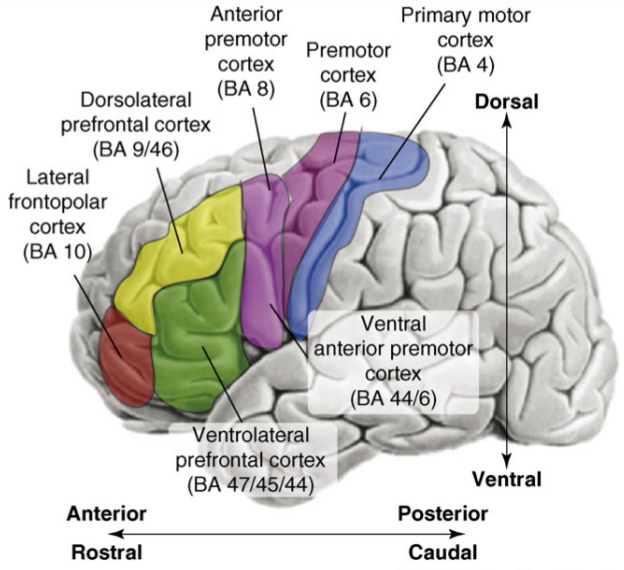
\includegraphics[scale=0.4]{figures/Badre08_1.png}
\caption{A lateral view on the PFC, with some of the most important areas highlighted. Note that PM and M1 (BA 6 and 4) are not considered to be part of the PFC. The ACC is located medially of the lPFC and can therefore not be seen in the figure. Reproduced from \citet{Badre2008}.}
\label{areas1}
\end{center}
\end{figure}

\subsection*{Functions}

The exact functions of prefrontal cortex and the best way to conceptualize these functions are still widely debated. However, thanks to numerous neuropsychological and neuroimaging studies, we do know that the general function of the prefrontal cortex is cognitive control (also known as the executive skills and the supervisory attentional function): influencing other processes in the brain based on its internal state. This includes at least planning, reasoning, problem solving, performance monitoring, attentional control, action selection, keeping track of goals, working memory and, last but not least, learning \citep{D'Esposito2002,Wood2003,Dayan2008,fuster2008prefrontal}. Note that these functions cover a large area of artificial intelligence research \citep{Russell1995}. We will first give a short overview of what is known about PFC function so far and then discuss action selection and attentional control in detail, as these functions are most relevant for our work.

As we discussed in the previous section, the PFC is not a homogeneous brain area. It has an intricate structure and different areas of PFC connect to different parts of the brain. This allows for easy hypothesis creation and testing in neuroimaging studies, which has quickly given us a general idea of the function of different areas. Ventromedial PFC has reciprocal connections with the amygdala and the hippocampus and indeed has been shown to be important for integrating emotions and memories with other information \citep{Bechara1999, Milad2007}. Lateral PFC on the other hand has reciprocal connections with the premotor cortex and the basal ganglia and indeed has been shown to be important for motor control, among many other cognitive control functions \citep{Ridderinkhof2004, Tanji2008, Goldman-Rakic2002, D'Esposito2002}. Another region that has received a lot of attention is the \gls{acc}, which is also connected with the dlPFC. It is thought that the ACC has the function to enhance control when performance is weak \citep{Silton2010}. Finally, the frontopolar cortex (BA10) is a large area at the front of the brain. Its function is largely unknown, although multiple proposals have been made \citep{Simons2006}. Please note that these results are neither exclusive nor definitive; the coming decades are bound to bring additional insights. 

So, we can find a general division of functions in the prefrontal cortex. However, it is not clear whether all these different brain areas with different functions do in fact function differently: it could well be that most prefrontal cortex function can be explained by one overarching principle, just applied to different domains (an influential example is the ``guided activation theory'' by \citet{Miller2001}). On the other hand, the PFC could be one large system that consists of different parts or not even one large system at all \citep{Simons2005}. At least for the learning in PFC, there is some hope that this can all be explained by dopamine-mediated reinforcement learning in combination with the basal ganglia \citep{Schultz2010}. Many research groups are working on this and much progress has been made the past decade \citep{Glascher2010, Botvinick2009}. One of the basic ideas is that dopamine encodes the prediction error for temporal difference learning. The dopamine is released in the \gls{bg} and is known to influence most of the PFC neurons. In this way, connections in the PFC can be adapted to better predict outcomes of actions in the future.

Another focal point in the debates about PFC is the way in which information is stored. This is an important point, because of the more theoretical interest in our reasoning and planning processes from both the psychology and the artificial intelligence community. One popular approach to studying the processing of information in the PFC is to define task sets. A task set is supposed to be a set of rules, encoded in the PFC, that can be used to solve a specific task \citep{Sakai2008}. The process of learning can then be described as the creation and consolidation of new task sets and task switching can be achieved by activating the new task set and deactivating the old task set. How this would be achieved exactly is another question; task sets by themselves are purely a psychological construct. The construct of task sets does explain many behavioural phenomena though, for example task switching phenomena like the ``switch cost'' \citep{Monsell2003}, explaining its popularity.

We will now focus on attentional control and action selection by lPFC, as those functions are most consequential to our research.

\subsection*{Action Selection and Attentional Control}

A good account of how attentional control could work is given by \citet{Miller2001}. In that article, it is proposed that the lPFC uses one mechanism, attentional control, to influence both the bottom-up flow of information and the activation of motor programs. An example of control over bottom-up information is visual attention research \citep{Rossi2009, Passingham2002, Morse2009}. Reducing the amount of incoming information is mainly important when many stimuli are present. The control over motor programs is also well-documented: mainly by the ideas of inhibitory control and for example go/no-go tasks \citep{Garavan1999, Mink1996}. This is mainly important when one stimulus has competing dimensions (for example in the Stroop task\footnote{Of course, attentional control does not necessarily have to work on motor programs in the Stroop task; it can also work on intermediate representations.}) or when very strong external stimuli are encountered. Thus, the ``guided activation theory'' from \citet{Miller2001} integrates a couple of psychological findings and gives us a simple, high-level description to lPFC function. An interpretation of the theory for a neural network is illustrated in figure \ref{MillerCohen}.

\begin{figure}[bthp]
\begin{center}
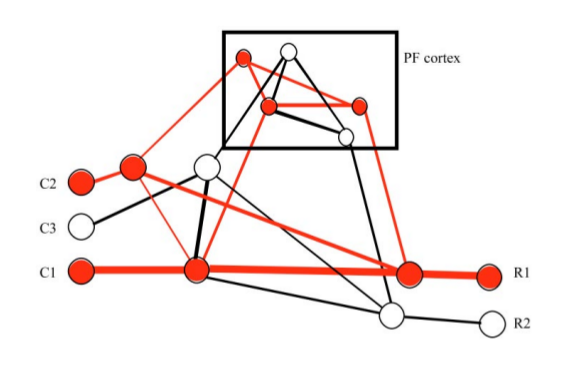
\includegraphics[scale=0.5]{figures/MillerCohen2001.png}
\caption{Attentional control by the neural networks in the PFC according to \citet{Miller2001}. At the left side, stimuli activate neurons. These neurons are coupled to response neurons at the right side. Without interference of the PFC, the stimuli only result in automated responses. Thanks to top-down connections from the PFC, these automated responses can be suppressed. The internal state of the PFC can for example be determined by the context of the situation, which asks for a different, non-automated response. Reproduced from \citet{Miller2001}. }
\label{MillerCohen}
\end{center} 
\end{figure}

\label{loops}
A very different view of prefrontal cortex function is obtained by investigating its anatomical connections with the basal ganglia that were mentioned before. Over the past decades, it has been found that these connections form loops, with output from the cortex to the Striatum, and input to the cortex trough the Thalamus. Between the Striatum and the Thalamus multiple connections have been found, involving the Globus Pallidus, Subthalamic Nucleus and Substantia Nigra. Other connections and areas are probably important as well \citep{Parent1995}. The hypothesized function of these structures is action selection \citep{Bogacz2007}. Apart from recordings of neural activity and lesions studies, one of the most interesting arguments for this hypothesis is that the BG are a very old brain region and that action selection is also one of the first problems an organism has to solve \citep{Redgrave1999} \footnote{Compare with the amount of effort spent on action selection for robots, e.g. \citet{Yamada1999}.}. The cortical loops that connect to the BG are then an extension or adaptation from older action selection mechanisms, to include the internal state (e.g. plans or beliefs) of the organism in the action selection process. How these loops function on a more detailed level is much debated though and an active area of research \citep{Prescott2006, Hazy2007}. In the literature review chapter, we will discuss an influential computational model, made by \citet{O'Reilly2006}. 

Our own research fits best in the tradition of \citet{Miller2001}, although the two points of view are not mutually exclusive. The guided activation theory is simply more abstract and does not make detailed predictions about the neural basis of the system. The ideas about cortical loops are very detailed in their anatomical description, but remain uncertain in the functional domain. Therefore, our own research can give results about general principles of PFC function, but is neither in agreement nor conflicting with evidence about the exact neural structures. One example of an attempt to reconcile the two approaches is \citet{Reynolds2009}, which will be discussed in the literature review chapter. 

We may conclude that we still have very much knowledge to gain regarding the PFC. Nevertheless, we can keep in mind that the PFC has an intricate structure that is responsible for most of the executive functions of the brain. One of these functions is to filter the bottom-up information stream and to control which motor programs are executed. This is probably mediated by the loops through the BG and PFC.

\section{Recurrent Neural Networks and Echo State Networks}
We will implement the model of the PFC with an Echo State Network. The basic concepts that are required to understand those networks are described here.

\subsection*{Recurrent Neural Networks}
Neural networks that allow connections between nodes to form cycles are collectively known as recurrent neural networks. Because of the cycles, recurrent neural networks can have an internal state that may influence the processing of new input in the network. This is in contrast with feedforward neural networks that will always process an input pattern in the same way regardless of its history. To keep track of all the connections, a recurrent network is usually defined by its weight matrix (or connectivity matrix). In this matrix the columns represent nodes from which connections originate and the rows represent the same nodes, but not on the receiving side of the connection. Thus, each element in the matrix represents the weight of one of the possible connections. This system is also described in figure \ref{weightmatrix}.

In an artificial recurrent neural network, we can now update the activation state of all the nodes in roughly the same way as in a feedforward network: at each node, we multiply the weights of all the incoming connections with the corresponding activations, sum these and apply an activation function (also known as the squeezing function) to get the new activation state. This can be summarized to the following equation, assuming that the activation function $f$ works on each element of the activation vector separately:
\begin{equation}
 \vec{A}_{\text{new}} = f(\vec{A}_{\text{old}} W + \vec{b} ) \label{update}
\end{equation}
with $\vec{A}$ the activation vector, $W$ the connectivity matrix and $\vec{b}$ the biases of the nodes.  

\begin{figure}[bthp]
\begin{center}
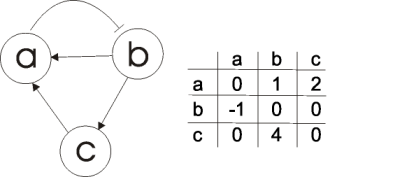
\includegraphics[scale=1.6]{figures/weightGraph.png}
\caption{A weight matrix for a recurrent neural network. When considering node b, we can find in the second column of the matrix that two connections originate there: one weak connection to node a and one strong connection to node c. We can see in the second row of the matrix that node b receives one inhibitory connection, from node a. Reproduced from the documentation of JCell \citep{Spieth2006}. }
\label{weightmatrix}
\end{center} 
\end{figure}

Note that although biological neural networks also show many recurrent connections, recurrent artificial neural networks are usually not even near approximating all the possible dynamics in biological neural networks. Therefore, most artificial neural networks can only be used for modelling of biological neural networks at a rather high abstraction level. However, some projects, like \citet{Pecevski2009}, specifically aim at modelling all the details of biological neural networks, such as neurotransmitter dynamics, dendritic potentials and synaptic plasticity. These simulations require too much processing power to be of practical use for more mundane applications unfortunately.

\subsection*{Training of Recurrent Neural Networks}
Apart from network dynamics, we obviously also need a way to mould these dynamics into a useful form. For the training of recurrent neural networks we have quite some possibilities. For supervised settings, meaning that we have a teacher signal for each moment during the training procedure, we can employ a gradient descent algorithm. The standard algorithm is 	``backpropagation through time'' (BPTT) \citep{Werbos1990}. A handful of other algorithms have been developed, for example ``real-time recurrent learning'' (RTRL) \citep{Williams1989}. All these algorithms suffer from the problem of vanishing error gradients though: when the dynamics of the network are near a bifurcation, a change in the weights may only lead to a tiny change in the results, slowing down the convergence of the algorithm considerably \citep{Doya1992}. 

A second option is an unsupervised learning algorithm. They have been used from the beginning of recurrent neural network research; Hopfield for example used Hebbian learning \citep{Hopfield1984}. It can deliver robust results for some specific applications. How to solve more problems with unsupervised learning algorithms remains an active area of research (e.g. \citet{Spratling2012}). The obvious disadvantage is of course that an unsupervised algorithm cannot guarantee a specific end result. 

There are still other options: particle swarm optimization \citep{Gudise2003}, simulated annealing, evolution \citep{Sexton1999} or reinforcement learning \citep{Lin1993}. Reinforcement learning uses feedback from the environment to strengthen actions that give high rewards and weaken actions that give no rewards. Although it is an interesting development and an impressive feat that it can be implemented in neural networks, it still has many problems: credit assignment is difficult in all but the most simple situations, unknown parts of the current state leads to perceptual aliasing, the explosion of the dimensionality and the use of discrete states and actions, etcetera \citep{Vlassis2012}. Two studies that investigate the link between abstractions and reinforcement learning are \citet{Frank2011} and \citet{Botvinick2009}.

Using evolutionary algorithms with neural networks is a field of research on its own as well (e.g. \citet{Yao1993, Kaiser2010}). The most basic approach is to directly encode every weight of a recurrent neural network in the genome. This research project in fact started off with an attempt at using this method. Two problems were encountered: firstly, when using a fully connected network, the genome quickly becomes far too long as the number of connections is quadratic with respect to the number of nodes. Secondly, the networks tend to fall into the ``holes of the fitness function'' before developing dynamics that are rich enough to solve the whole problem. The result of a long evolutionary run can for example be a network that always picks one output, regardless of the input. This second problem might be solved by following the advice of \citet{Beer1995} and ``anchoring'' the search to certain networks that only need small changes to show rich dynamics, but this was not investigated in this study. Nevertheless, some researchers manage to get good results with this most basic method, e.g. \citet{Paine2005}. 

More sophisticated methods of using evolutionary algorithms with recurrent neural networks have of course been developed. A good example to illustrate this is neuroevolution of augmenting topologies (NEAT) \citep{Stanley2002}. Instead of changing the connection weights in a fixed topology, the genotype in NEAT represents the topology as well. This allows to develop more complex neural networks from simpler ones and even different topologies that perform better at different aspects of the task. Another noteworthy line of research is Evolino \citep{Schmidhuber2007}, employing so-called long short-term memory (LSTM) networks \citep{Hochreiter1997, Gers2001}. The LSTM networks are yet another approach at improving gradient-based learning algorithms for recurrent neural networks, by enforcing that the network consists of very specific building blocks. Evolino is the evolutionary extension of this approach to increase the number of tasks that LSTM networks can be used for. After all, for LSTM networks the same is true as for all other recurrent neural networks: it will not achieve a good performance on all tasks.

Unfortunately, even with such a large number of training methods, the results are not satisfactory for all problems. While recurrent neural networks are universal dynamics approximators in theory \citep{Beer1995}, in practice they fail at many tasks. Therefore, new methods of using recurrent neural networks are still being developed. One of these (rather) new methods is Reservoir Computing.

\subsection*{Reservoir Computing}
Reservoir Computing (RC) is one of the answers to the problems of recurrent neural networks with supervised learning. When using this method, the recurrent neural network itself is referred to as the ``reservoir'' and is not trained at all. Its only function is to combine the inputs with its internal state, effectively mapping the inputs to the high dimensional space of the network state (similar to the kernel trick, e.g. \citet{Baudat2001}). The network state is then fed into a perceptron and we try to get the desired output by setting the weights of the perceptron, which can even be done with linear regression. Sometimes feedback connections from the perceptron to the reservoir are used to achieve more stable dynamics \citep{Lukovsevivcius2009}. In figure \ref{ReservoirComputing} the idea of reservoir computing is visualized. 

\begin{figure}[bthp]
\begin{center}
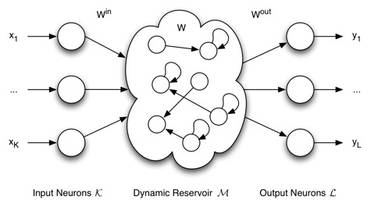
\includegraphics[scale=0.6]{figures/reservoir.jpeg}
\caption{The principle of Reservoir Computing: the input is fed into a non-linear dynamic system and the weights to the output neurons are trained to obtain the desired results. In this case, multiple output units are defined, but feedback is lacking. Reproduced from \citet{Oubbati2010}. }
\label{ReservoirComputing}
\end{center}
\end{figure}

Interestingly, multiple versions of reservoir computing have been developed independently, with the two best known versions being the Echo-State Network (ESN) by \citet{Jaeger2001} and the Liquid State Machine (LSM) by \citet{Maass2002}. However, the first to apply the idea of Reservoir Computing was \citet{Dominey1995}. In fact, his research has so much in common with our own that we will discuss this article and a recent follow-up \citep{Hinaut2011} in the literature overview. Here we will just describe the ESN and the LSM to understand the basic principles of Reservoir Computing.

The ESN utilizes simple perceptron-type nodes in its reservoir and is therefore computationally relatively cheap. Its name derives from the ``echoes'' of the input patterns that should be available in the network for readout. It gives better performance than other types of recurrent neural networks on a couple of tasks, most notably time-series prediction (non-linear autoregressive moving
average (NARMA) timeseries), e.g. \citet{Jaeger2004}. From the neuroscience perspective, its main disadvantage is the lack of biological plausibility. The LSM on the other hand mostly uses spiking neurons and is much more related to accurate models of biological neurons. Its name derives from the analogy of the reservoir with a basin that is perturbed by something falling in. Because of the use of spiking neurons, rich dynamics can be achieved with a reasonably small number of neurons. The main disadvantage of the LSM is its computational cost, especially when more realistic neuron models are used. Some work has been done to use a physical reservoir instead of a software reservoir to address this problem, e.g. \citet{Paquot2012}. For an in-depth review of reservoir computing techniques, see \citet{Schrauwen2007}.

For reservoir computing to work, the reservoir should have some special properties. First of all, the dynamics of the network should not be chaotic: it would make the current state of the reservoir only dependent on the connectivity instead of on the past input patterns. The network state should also not only depend on the current input: the past input should still have a noticeable effect on the network activity. This is referred to as the input separability of the network. Thus, we need a reservoir that has a slowly fading ``echo'' of inputs. In the ESN, this is called the Echo-State Property (ESP). For simple echo state networks it has been shown that setting the spectral radius (which is the largest eigenvalue) of the connectivity matrix smaller than one is a sufficient condition to obtain the ESP. The precise setting of the spectral radius determines for which tasks the reservoir will perform best \citep{Jaeger2001}. 

This is in fact one of the weak points of reservoir computing: every application requires tweaking of the reservoir. This point will be discussed further in the literature review chapter. Nevertheless, thanks to reservoir computing the domain of tasks that can be solved with recurrent neural networks is extended a little bit more again, because it alleviates the difficulties with training them. One of the tasks that ESNs can be used for is classification, which is why we chose to use this class of recurrent neural networks.

\section{Embodied Neuroscience and Robotics}
For the construction of our model, we will keep application of the model for a robot in mind. This serves two purposes: first of all, we may be able to contribute to adaptive behaviour research with inspiration from neuroscience. Secondly, a robot implementation can give new insights about the functions of the PFC and the development of the PFC during evolution, by allowing investigation of real-life situations instead of the well-known psychological task battery. We will here discuss the theoretical background of neuroscience employing robots.

\subsection*{Embodied and Embedded Cognition}
Nowadays, cognitive sciences usually do not focus on the brain or control architecture of an agent in isolation any more, but in combination with the body and/or environment. In other words, cognitive sciences used to have a cognitivist approach, but embodied and embedded (aka situated) cognition (EEC) has gained influence \citep{Dijk2008}. Still, the exact meaning of embodiment and situatedness is not yet crystallized to a standard definition. As I would like to argue that the proposed control architecture is in fact in compliance with the EEC paradigm, it is important to investigate the exact meaning of those concepts. 

\begin{figure}[bthp]
\begin{center}
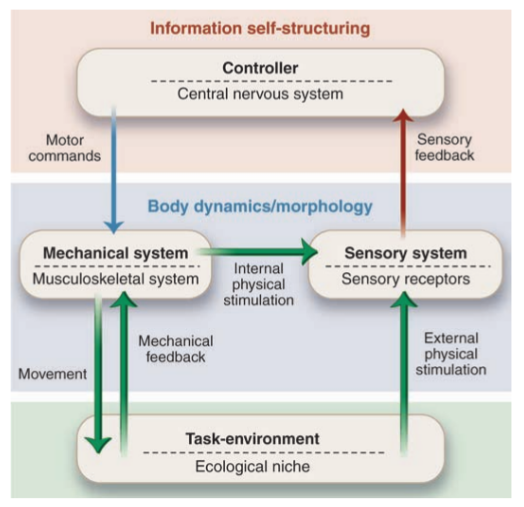
\includegraphics[scale=0.5]{figures/EEC.png}
\caption{The interactions between the brain (the top layer), the body (the middle layer) and the environment (the bottom layer). Instead of considering the brain in isolation, a better description may be obtained by investigating the body and the environment of a subject as well. Reproduced from \citet{Pfeifer2007}. }
\label{EEC}
\end{center}
\end{figure}

Situatedness means that we are interested in an agent that deals with an environment. In case this environment is static, the agent can gather as much information about the world as necessary and then leisurely make a plan of action, as in the old sense, plan and act (SPA) approach. Most real environments are not static though, introducing time constraints on the control architecture. This means that agents have to make decisions and act without complete information and moreover, without too much planning (corresponding with the situated, time-pressured and action-based cognition in \citet{Wilson2002}). Thus, an effective controller has to take the properties of its environment into account.

Embodiment means that an agent has a body: a physical implementation of all its components in this world and therefore also a means of interacting with the world \citep{Pfeifer2007}. \citet{Ziemke2001} tries to give a broad classification of the possible types of embodiment. Obviously, different means of interacting with the environment lead to different behaviours and control strategies. An efficient controller should therefore also be adjusted to the body of the agent as well as to the environment. For our model, this immediately leads to an important requirement: it should be computationally cheap, as we cannot fit a robot with a supercomputer.

Combining the notions of embodiment and situatedness leads to even more consequences. One of the most important results is a possible solution for the grounding problem in GOFAI (good old fashioned artificial intelligence). See the Chinese room example in \citet{Ziemke2001} for an illustration of this problem. EEC gives a solution to this problem because concepts can now be coupled with the real world through sensations and actions. In this thesis grounding will not be central, so for a review about this I direct the reader to \citet{Barsalou2008} and \citet{Anderson2003}. This corresponds to the body-based cognition that Wilson discusses.

The most extreme interpretation of EEC is that it is actually a mistake to make a boundary between the controller, body and environment of the agent, because the links between those three are as important as the links within them. This is the concept of the ``extended mind'' \citep{Clark1998} (which is listed as the fourth interpretation in the article by Wilson). This interpretation is very interesting indeed, but many argue that it is too extreme. A less extreme version of this idea is that cognition is a result of the interactions between controller, body and environment, for example in the case of offloading cognitive work onto the environment, which alters the task that the controller has to perform (which Wilson splits into her first and third interpretation) \citep{Haselager2008}. 

Another important example of cognition arising from interplay between controller, body and environment is a new way to look at perception. Instead of only passively examining the input of our sensory system, we can also imagine active perception now: using actuators to control what is perceived. One can argue that active perception is in fact used all the time by animals, for example when we track an object with our eyes. \citet{Nolfi2002} does a good job at explaining how powerful active perception can be and how it can solve the aliasing problem. This problem is the result of the fact that a purely reactive agent will always do the same thing in reaction to the same sensory input. So, what will this agent do if the same sensory input can mean two things? The EEC answer is that this agent should look for more information, which can be done thanks to its actuators. In other words, ``the world is its own best model'' \citep{Brooks1991}. This is in contrast with a SPA agent, which would solve the aliasing problem by investigating its world model (for example, choose the solution with the highest probability or build a plan to solve this problem).

As we can now see, it is known that action selection and cognitive control in general cannot be fully explained by only looking at the reaction times of artificial tasks. This notion has not reached very far in neuroscience yet, even though the idea has been around for a long time already \citep{Chiel1997}. We will attempt to make a step in this direction by preparing for a robot implementation of our model.

\subsection*{Robot Control}
In robotics, the embedded and embodied paradigm is quite important since Brooks criticized the sense-plan-act (SPA) class of robot controllers for its emphasis on symbolic planning \citep{Brooks1991a}. The main problems with SPA architectures are the amount of resources that is required in the planning stage and the difficulty of building the accurate world model that is necessary for planning. Due to the large number of dimensions in even a quite simple environment, making a plan to achieve certain goals can takes a very long time. All this effort is wasted if the world model turned out to be inaccurate or if the environment has changed in the meantime. One way to solve this problem is to improve the planning stage; we will not discuss this line of research here, but see for example \citet{Schut2001}. Another solution is to do away with planning: \citet{Brooks1991a} proposed to use reactive robots instead: robots with a control architecture that does not keep an internal world model and does not make plans.

A good example of a reactive robot architecture is the subsumption architecture, which improves on the simplest reactive stimulus-response mappings. The subsumption architecture consists of layers with simple behaviours (rather tight input-output couplings), in which higher layers can block lower layers. It can be argued that this mimics the way in which humans and animals perform simple, but intelligent, behaviour. However, this approach has two problems: firstly, when increasing the number of layers, there is no structured way of arranging the inhibition to attain the desired complex behaviour. This can be countered by using evolutionary algorithms \citep{Koza1994}, but this has never been demonstrated to be able to handle more complex situations\footnote{Common strategies in evolutionary algorithms, incremental and modular evolution, are not guaranteed to work for the same reasons as design by hand cannot handle complex situations while designing subsumption controllers: it is not always possible to find a subdivision of tasks that are unrelated and can therefore be designed or evolved independently.}. Secondly, the subsumption is all-or-nothing in its inhibition, while some situations are better dealt with by integrating information in a continuous fashion and some situations require lower layers to overrule higher layers. In other words, information is lost because of higher layers inhibiting lower layers \citep{Rosenblatt1989}.

Over the years, two acceptable and useful methods for robot control were developed: hybrid architectures and behaviour-based architectures. Hybrid systems have a reactive bottom layer for fast, time-critical responses and a symbolic top layer for long-term planning and the monitoring of progress. A middle layer is necessary to combine these two antagonists, and that is were most effort is focused \citep{Gat1997}. Note that such systems still have the problems that planning effort may be wasted. For this thesis, behavioural systems are more important: the direct descendants of the subsumption architecture, the control system consists of a number of behaviours. These behaviours are allowed to influence each other as well as the motor output. Some of the behaviours can also be used to store information about the environment, like a map for example. Note that such a controller still lacks proper design principles for complex behaviours and the way in which behaviours should influence each other \citep{Arkin1998}. A recent, flexible implementation is IB2C, which is illustrated in figure \ref{ib2c} \citep{Proetzsch2010}.

\begin{figure}[hbtp]
\begin{center}
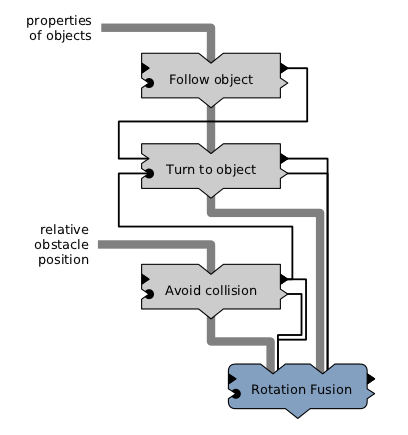
\includegraphics[scale=0.4]{figures/ib2c.png}
\caption{ A fragment of a behavioural robot control system based on IB2C. The fusion behaviour in the bottom of the figure collects turning suggestions from the other behaviours and uses these suggestions to decide on the actual motor commands. Inhibitory, excitatory and data connections are explicitly separated. Reproduced from \citet{Proetzsch2010}.}
\label{ib2c}
\end{center}
\end{figure}

In \citet{Scheutz2004} a useful classification of behaviour-based control architectures is given. The first distinction is the way in which the action selection is handled. Action selection is simply the decision which action should be executed at a certain moment, while there may be many competing proposals. This can be solved in a cooperative and competitive way. In the competitive case, the different behaviours compete with another, and the winner decides what command is issued to the actuators. Subsumption is the obvious example. Cooperative architectures on the other hand include a way to achieve command fusion (or behaviour fusion). This can be implemented with a voting system, fuzzy logic, simple addition or in still other ways. The second distinction is between adaptive and non-adaptive systems. Adaptive architectures allow for adjustment of behaviour selection strategies during the lifetime of a controller instance \citep{Wareham2011}. Most architectures do not support such an adjustment however and are called non-adaptive, of course. 

Finally, we have to note that not all robot controllers are part of the classes described above. Most notably, a large number of robot controllers are based on artificial neural networks and more or less inspired by neuroscience \citep{Lin1993, Erlhagen2006}. Often, the design of neural networks for low-level control is obtained with artificial evolution \citep{Floreano2000,Baldassarre2009,Fernandez-Leon2009}. Unfortunately, such controllers are in general hard to use again on different robots, on different tasks, or to built more complex behaviours. Interestingly, only a few robot controllers are explicitly inspired by models of cognitive control; probably due to high computational demands of existing models. The few examples will be discussed in the next chapter. 

We can conclude that most natural tasks of the human brain are probably not quite like the tasks that are in general used for psychology and neuroscience research: the brain is embodied and embedded, which is often ignored in experiments. One of the methods to extend neuroscience to situations in daily life is to use robots. Therefore, we will keep the application of our model in a robot in mind.

\chapter{Literature Review}
In this chapter we will discuss the articles that are particularly relevant for this thesis in more detail. 

\section{Topological Mapping of Abstractions}

\subsection*{Hierarchy and Abstraction} 
Our efforts are in line with a long tradition of research into hierarchical structures in behaviour and in the brain. Hierarchies of different abstraction levels are required, because low-level information is too high-dimensional to take everything into account at higher planning, association and learning levels \citep{Lashley1951}. Note that without planning and abstraction, it seems possible to learn only automated stimulus-response mappings (see \citet{Dayan2009} for a review about the difference between rule-based learning and learning of automated responses). Numerous examples of hierarchical structures can be found in both human behaviour \citep{fuster2008prefrontal} and in brain structure, see figure \ref{fusters}. A simple example is the way in which we can interchange or adapt small chunks of behaviours that we learned earlier to create new behaviours, e.g. learning to make a sandwich with tomatoes after having learned how to cut tomatoes and how to make a sandwich with cheese. Two important reviews on the subject of abstractions are \citet{Badre2009} and \citet{Botvinick2008}. We will follow the first in the identification of four types of abstraction for regulation of behaviour: domain generality, relational integration, policy abstraction and temporal abstraction (of which the last two are also identified by \citet{Botvinick2008}). 

\begin{figure}[tbhp]
\begin{center}
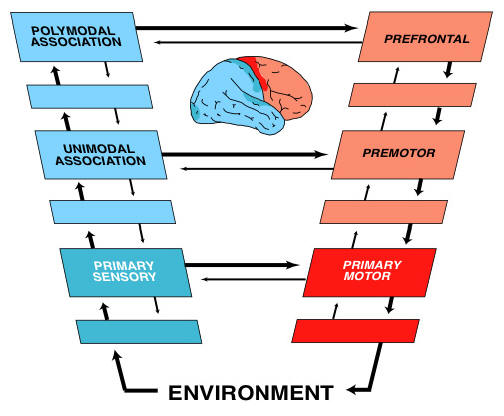
\includegraphics[scale=0.5]{figures/Cortical_Memory_fuster_f2.jpeg}
\caption{Fuster's hierarchy of brain structures, with fast and simple perception-action loops at the bottom and slow and complex perception-action loops at the top. Reproduced from \citet{Fuster2002}.}
\label{fusters}
\end{center}
\end{figure}

When the brain deals with representations that do not concern only exactly this moment in time, but a longer time period, this is known as temporal abstraction \citep{Fuster2001, Kiebel2008}. This concept is very close to working memory when studying the PFC. In the sandwich case, temporal abstraction is required to keep the goal of making a sandwich in mind while cutting the tomatoes. It is also important for the correct execution of action sequences, as is for example discussed in \citet{Elman1990}. Tasks testing temporal abstraction are the n-back test, 1-2 AX-CPT, which is an extension of the AX version of the continuous performance task, and the Store-Ignore-Recall (SIR) task \citep{Osaka2009, O'Reilly2006}. In the AX-CPT, participants are required to give one response to all trials, except when the preceding trial showed an A and the current trial shows an X, in which case a different response has to be given. In the SIR task, digits are shown in either red or black. In case the digit is black, it should be read aloud but otherwise ignored (ignore). In case the digit is red, it should be read aloud and kept in memory (store). Sometimes, an x is shown instead of a digit, prompting the participant to say which digit he recalls (recall).

Situations involving temporal abstraction often also involve policy abstraction\footnote{Probably due to the fact that a person is in general doing only one thing at a time.}. Policy abstraction describes a relation between goal representations in which the higher goal representation does not deal with motor commands directly, but only with other goal representations at lower levels. Again, this type of abstraction is encountered in the example of making a sandwich: the goal of having something to eat does not give you any information about the motor commands that should be used to achieve this goal. However, it does influence lower level goals, like finding bread and cutting tomatoes, that do give motor commands. Moreover, it also prevents distracting information to influence your behaviour: it could for example stop you from picking up that interesting book that you still wanted to read. The Wisconsin Card Sorting (WCS) task is a test for this abstraction type: the participant is shown cards with symbols that vary in three dimensions: color, shape and quantity. The cards have to be sorted according to one of these properties, while ignoring the other properties. Not relevant for policy abstraction, but included in WCS, is that the participant has to find out which dimension is relevant from error feedback.

Relational integration is the name for the relationships between representations. At the lowest level, this could for example be a property of an object. At higher levels we can make comparisons between concrete properties and compare relationships. A task testing this abstraction is for example a match/non-match task. Finally, domain generality refers to representations that are used over different (input) domains. For example, ``cutting'' neurons can be active when making a sandwich, but also when preparing dinner. Therefore, the cutting representation is more abstract than the cutting bread and cutting fish representations. A test for domain generality could for example be a task in which a left-hand response has to be given after hearing a sound and smelling something, while a right-hand response has to be given after seeing or feeling something.

In the same review, \citet{Badre2009} discuss the structural organization of the PFC. Based on anatomical evidence from \citet{Petrides2007}, they argue that we can find a hierarchical structure with the FPC at the top, the dlPFC and vlPFC in the middle, and at the bottom PMd and PMv that in turn connects to M1. This structure is clarified in figure \ref{PFCHierarchy}. Thus, we can find a hierarchical structure in the anatomy of the human PFC and a hierarchical organization of perception and behaviour in the functional domain. However, it is very important to note that this does not necessarily mean that the levels of both organizations map onto each other topologically. For example, it could be possible that all information that is more abstract than basic motor programs is processed in dlPFC. Therefore, we will now discuss the evidence regarding a topological mapping over the PFC.


\begin{figure}[bthp]
\begin{center}
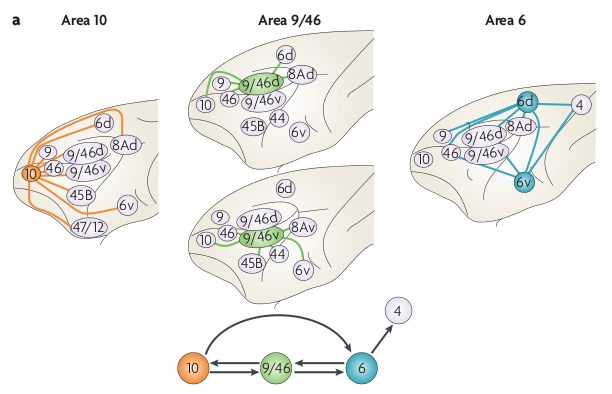
\includegraphics[width=\textwidth]{figures/PFChierarchy.png}
\caption{ The FPC (BA 10), lPFC (BA 9/46), PM (BA 6) and M1 (BA 4) form a hierarchical system, with separate ventral and dorsal branches. Reproduced from \citet{Badre2009}. Note that both \citet{Koechlin2007} and \citet{Badre2007} propose an extra level of abstraction in posterior lPFC or BA 8, between anterior lPFC and PM.}
\label{PFCHierarchy}
\end{center}
\end{figure}


\subsection*{Evidence for a Topological Mapping}

By now, multiple research groups have reported that different levels of abstraction map topologically to different areas in the human PFC, with higher abstraction levels mapping to more anterior regions. Before these results were found, some information was already available from primate studies (e.g. \citet{Petrides1991} in which dlPFC and PM lesions are distinguished by the influence on simple tasks: PM lesions gave problems with domain specific motor tasks while dlPFC lesions gave problems with a domain general monitoring task). One of the first publications proposing a rostrocaudal hierarchical organization in human PFC is \citet{Christoff2000}. This article contains a review of fMRI studies in which FPC or lPFC are activated, and proposes that the dlPFC is recruited for the evaluation of externally generated information, while the FPC is recruited when internally generated information (e.g. information in the dlPFC) has to be evaluated.

Not much later, specific studies were conducted to test these ideas directly. One very influential fMRI study is \citet{Koechlin2003}. The task that was used consisted of trials in which the participant had to give a motor response on simple visual input. Three abstraction levels were investigated by varying the number of possible motor responses, the amount of information given by a context cue and the amount of information given by an instruction cue in the beginning of a block of trials. Varying the first factor resulted in differential activation in PM, varying the second factor caused differential activation in caudal lPFC and varying the episode factor activated rostral lPFC. This is evidence for a topological mapping of policy and temporal abstraction (note that the article uses the terms contextual and episodic abstraction instead). Evidence for a hierarchical cascade was given by structural equation modelling. 

A couple of research groups replicated the findings from \citet{Koechlin2003}, but all in a slightly different way. We will discuss the most important studies here. \citet{Badre2007} varied the amount of competition on the response level, the feature level (which is policy abstraction), and additionally, the dimension and temporal level. The dimension level is a relational abstraction over the features, and the temporal level (which is called ``context'' level in the article, not corresponding to the context from \citet{Koechlin2003}) consists of episodes with particular mappings of the dimension level. This is illustrated in figure \ref{taskBadreReynolds}. The fMRI result for these four levels of abstraction was that PMd, caudal lPFC, rostral lPC and FPC were respectively activated, reasonably matching the results from \citet{Koechlin2003}, see figure \ref{BadreKoechlin}. \citet{Krawczyk2011} also obtained similar results with relational integration abstractions.

\begin{figure}[bthp]
\begin{center}
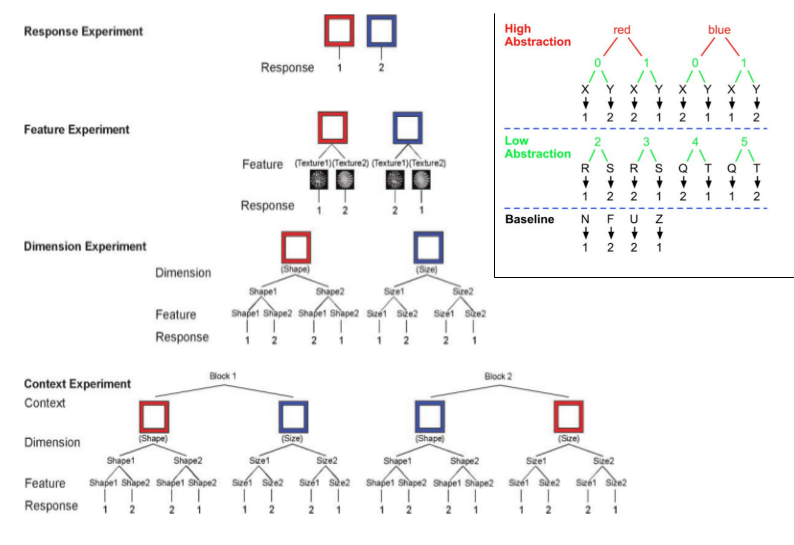
\includegraphics[width=\textwidth]{figures/taskBadreReynolds.png}
\caption{The tasks used in \citet{Badre2007} and \citet{Reynolds2012} (inset). The dimension experiment and the high abstraction task can be represented in the same tree structure, but may be solved differently by humans due to the different use of abstractions: in the dimension experiment, relational integration is used as well as policy abstraction, while only policy abstraction is used in the high abstraction task. Reproduced from \citet{Badre2007} and \citet{Reynolds2012}. }
\label{taskBadreReynolds}
\end{center}
\end{figure}

\begin{figure}[bthp]
\begin{center}
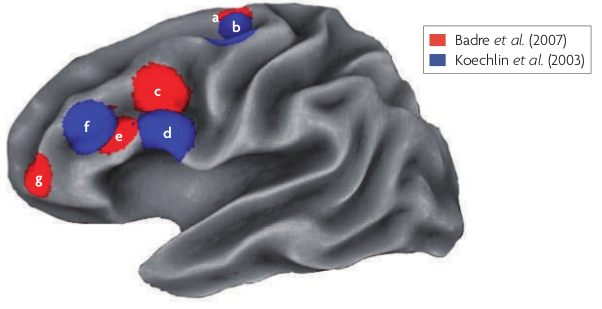
\includegraphics[width=\textwidth]{figures/BadreKoechlin.png}
\caption{The results of \citet{Koechlin2003} compared with \citet{Badre2007}. While the subsequent abstraction levels give activation in similar areas, it is not clear whether the results from the two articles are the same. Reproduced from \citet{Badre2009}. }
\label{BadreKoechlin}
\end{center}
\end{figure}

\citet{Christoff2009} chose to use words instead of simple visual cues in their experiment, to directly test abstraction effects while controlling for the possible confound of task difficulty in the other studies. The participants had to solve five- and six-letter anagrams of words with a meaning of low, medium and high abstraction. While the behavioural results were exactly the same over these three categories, the fMRI results showed differential activation in respectively the ventral PFC, dorsal PFC and rostral PFC. See figure \ref{christoff} for a more exact localization.

\begin{figure}[bthp]
\begin{center}
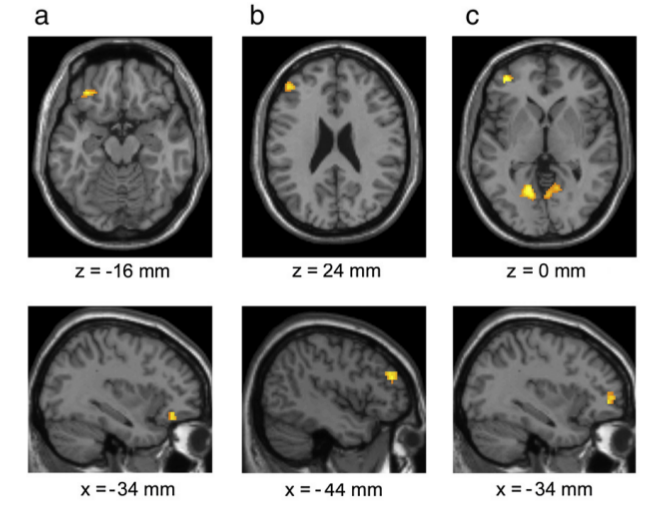
\includegraphics[width=\textwidth]{figures/Christoff.png}
\caption{The results from \citet{Christoff2009}. Anagrams with low abstraction showed activation in ventral PFC (a), anagrams with medium abstraction in dorsal PFC (b) and rostral PFC was activated in the most abstract cases (c). Reproduced from \citet{Christoff2009}. }
\label{christoff}
\end{center}
\end{figure}

The most recent addition to the collection of fMRI results is by \citet*{Reynolds2012}. The different abstraction levels were compared directly with each other in five conditions: baseline, low temporal and policy abstraction, high temporal and low policy abstraction, low temporal and high policy abstraction and finally high temporal and high policy abstraction. The low temporal conditions match more or less with the first two abstraction levels of \citet{Badre2007} (see figure \ref{taskBadreReynolds}), and the high temporal and high policy abstraction condition matches more or less with the third abstraction level of \citet{Badre2007}. The high temporal abstraction and low policy abstraction matches with the episode factor from \citet{Koechlin2003}, while his policy factor is similar to the low temporal abstraction and high policy abstraction condition. The results for a particular region of interest in dlPFC are that it is least active in the baseline condition, shows most activity in the high temporal and high policy abstraction condition and shows comparable intermediate activity in the other three conditions.

Finally, for those not convinced yet, a lesion study also provided evidence for a topological mapping of abstraction on the PFC \citep{Badre2009a}. On a similar task as in \citet{Badre2007}, described above, the reaction times of subjects without lesions and subjects with lesions at different locations were compared. The results were that a lesion at a location impairs a specific abstraction level, but also higher abstraction levels. These results were obtained by finding weak correlations in a group of only twelve patients however, indicating that we should still take some care with the interpretation. Nevertheless, the results were significant, making it proper evidence for an actual hierarchical organization instead of just a topological mapping.

\subsection*{Theories for Topological Mapping}

These convincing results have led to a number of theories. The study by \citet{Petrides1991} suggested domain specific neurons to have a different location in the PFC than domain general neurons, but this has not been tested in humans. \citet{Koechlin2003} proposes a ``cascade'' model of cognitive control, with more anterior regions influencing posterior regions step by step. This is illustrated in \ref{Koechlin}. This theory is backed up by information theoretical measures (mainly mutual information and entropy), although it seems almost impossible to investigate these measures in the brain, apart from correlating it with fMRI activity or reaction times \citep{Koechlin2007a}. Due to the explicit notion of episodic control, a large part of this theory is based on the handling of temporal abstraction \citep{Koechlin2007}. However, the contextual information in the cascade model matches policy abstraction.

\begin{figure}[bthp]
\begin{center}
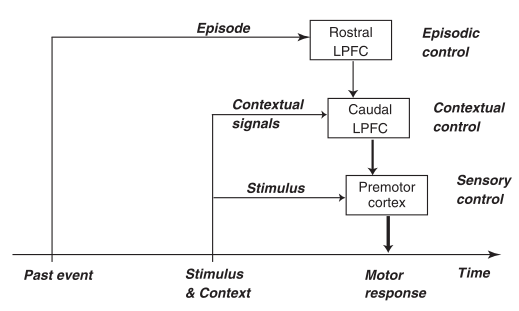
\includegraphics[scale=0.5]{figures/koechlin.png}
\caption{The cascade model in which more anterior regions influence posterior regions in a cascade of cognitive control. Reproduced from \citet{Koechlin2003}. }
\label{Koechlin}
\end{center}
\end{figure}

\citet{Badre2007} proposes a theory that is related to \citet{Koechlin2003}, by stating that the functional gradient in the PFC might be explained by increasing abstraction levels in general, and in particular increasing levels of policy abstraction. Just like \citet{Koechlin2003}, \citet{Badre2007} implicates FPC, lPFC and PM in this hierarchy. \citet{Christoff2009} suggests that for relational integration, the set of areas in the hierarchy are slightly different: the highest abstraction levels are again mapped onto the FPC (in line with \citet{Christoff2000}), but the middle and lowest level are mapped onto respectively the dlPFC and vlPFC. This difference might be explained by the use of words instead of simple visual cues in the task. 

\citet{Reynolds2012} used their own neuroimaging results to make yet another proposal: the ``adaptive context maintenance'' hypothesis. According to this hypothesis we should not assume a hierarchical, rostrocaudal organization. Instead, we should be able to find both posterior and anterior PFC activity for the duration that contextual information had to be maintained to perform a task. Indeed, the imaging results they present do not seem to match the previous two theories and can be explained by adaptive context maintenance only. The article presents this hypothesis as an alternative for the two theories discussed above, but may misguide the reader by doing so. \citet{Koechlin2003} and \citet{Badre2007} do namely not discuss the way in which information is maintained or updated and therefore do not contradict \citet{Reynolds2012}; in fact, ``adaptive context maintenance'' may even be a logical extension to their theories. What remains is a neuroimaging result that cannot be explained by the cascade theory or by abstraction levels, but this could be caused by differences in the paradigm (e.g. the region of interest or the particular task that was used). Therefore, this hypothesis seems to be orthogonal to the two theories about rostrocaudal organization. The question that remains is whether \citet{Reynolds2012} are right about the absence of a hierarchical organization; our results will contradict this.

It is important to notice some subtle differences in the tasks of \citet{Koechlin2003}, \citet{Badre2007} and \citet{Reynolds2012}. \citet{Koechlin2003} uses a task similar to WCS for their policy factor: the context cue is used to choose one out of two relevant stimulus dimensions. \citet{Badre2007} on the other hand use their second level of abstraction (feature level) only to invert the stimulus-response mapping. Then, in their third abstraction level, the policy abstraction is replaced by relational integration and the extra level of abstraction is a policy abstraction as in \citet{Koechlin2003}. \citet{Reynolds2012} use the two policy abstraction levels for inverting the stimulus-response mappings. They also show that the task can be represented in a tree in the same way as the third abstraction level of \citet{Badre2007}; see figure \ref{taskBadreReynolds}. However, this does not mean that the human participants solve the task in the same way: in fact, the differences between abstractions is one of the questions that is posed in \citet{Badre2009}. A second problem is that the use of policy abstraction to invert a stimulus-response mapping is not intrinsically abstract: the ``abstract'' cue gives just as much information about the response as the ``less abstract'' cue. Therefore, participants may solve this task without using two levels of abstraction\footnote{An alternative strategy for the task in \citet{Reynolds2012} would for example be: start with having in mind a right hand response. Switch if the first cue is blue, do not switch if red. At the second cue, again, switch if 0, do not switch if 1. At the third cue, switch if X, do not switch if Y. If the WCS task would have been used, as in \citet{Koechlin2003}, such a strategy would have been much less efficient than a strategy using abstraction levels.}. All in all, it is not surprising that the results show differences. This also means that until more these uncertainties are resolved, we cannot directly use the imaging results to construct a detailed model of PFC.

Considering the different proposals, the research groups seem to have matched their theory to the specific task that was used in the imaging experiments. This brings up the important question how the fragmented experimental results and theories are related to each other and how we can best describe the structure in PFC. In particular, we would like to investigate whether mapping of temporal and policy abstraction can be explained by the task requirements of information integration and preservation. To do so, we turn to a computational model.

\section{Computational Models of Prefrontal Cortex}

Computational models related to the PFC have quite a long tradition (see \citet{Botvinick2008} and \citet{O'Reilly2010} for an overview). Historically, the most important distinction is between symbolic models and connectionist models. Symbolic models perform their function by using symbols for concepts. Whether such a model performs action sequencing or reasoning, and whether it is a neural network or a searching method, we can always pinpoint one part of the model which defines the concepts that are used. In connectionist models this is not the case: the used concepts are only described by a particular state of the system; usually an activation or connection pattern in a neural network \citep{Rumelhart1986}. 

First of all, we cannot write about computational models of the PFC without mentioning cognitive architectures. These grand architectures aim to mimic all aspects of human cognition or even consciousness. Their roots in GOFAI gives most of them a solid symbolic foundation with elaborate logic and planning schemes. A good example is ACT-R (Adaptive Control of Thought - Rational). It has been used to simulate cognitive tasks and recently, also to predict fMRI results of these tasks \citep{Anderson1997}. One other cognitive architecture that is interesting is LIDA (Learning Intelligent Distribution Agent). This architecture is not purely symbolic and in fact incorporates some ideas from EEC. It includes a notion of consciousness and can be considered an implementation of Global Workspace Theory (GWT) \citep{Baars2009}. Unfortunately, their computational requirements do not make cognitive architectures a good candidate for autonomous robot control, and we will not discuss these models any further. 

Instead, we will describe more focused, neuroscience based models of PFC. These can roughly be divided into four areas: performance monitoring and error detection \citep{Alexander2010}, the (expected) reward and reinforcement learning \citep{O'Doherty2003}, working memory in the PFC and BG \citep{Hazy2007} and models about action sequencing and action selection \citep{Botvinick2008}. We will describe the studies that include ideas about the hierarchical organization of PFC.

\subsection*{Hierarchical Models of PFC Function}

Hierarchical models of PFC function used to be mainly models of action sequencing \citep{Allen2010, Dayan2009}. They can be divided into instrumental and correlational models. Instrumental means that the control rules are encoded as means-ends relationships (e.g. I want to drink, thus I pick up a cup) while correlational means that only the transition probabilities are encoded (e.g. I want to drink, and drinking usually happens when picking up a cup). An example of an instrumental model is presented by \citet{Cooper2000}. They show that their model is capable of organizing sequential, hierarchical behaviour based on precoded action schemas. This is achieved in situations with about ten low-level actions and about ten hierarchically organized high-level goals. They also argue that the errors in their model in noisy conditions resemble human errors, although this is not quantified. Also note that hierarchical behaviour is not necessarily linked with a hierarchical PFC. \citet{Uithol2012} gives an elaborate and insightful treatise on this subject, explaining how temporal abstraction relates to action sequences.

The link between hierarchical behaviour and a hierarchical PFC is partly established by \citet{Botvinick2004}, in agreement with the ideas from \citet{Uithol2012}. They present a connectionist, correlational model that does not require hierarchical schemas. Instead, the continuous time recurrent neural network is trained by BPTT on a hierarchical task and learns to perform it. An extension of this model that is very relevant for us, is given in \citet{Botvinick2007}. Here, the CTRNN is assumed to have a hierarchical structure and trained on a Store-Ignore-Recall (SIR) task and an action sequence, which have multiple timescales. This includes policy and temporal abstraction. Thanks to the structure of the task, it is possible to assess which part of the network processes the longer timescales. As we might expect by now, it turned out that the longer timescales were handled by the top part of the network (note that the time constants were the same throughout the network). Thus, in this model the levels in the action hierarchy are in fact coupled to the hierarchy in the network topology.

\begin{figure}[tbhp]
\begin{center}
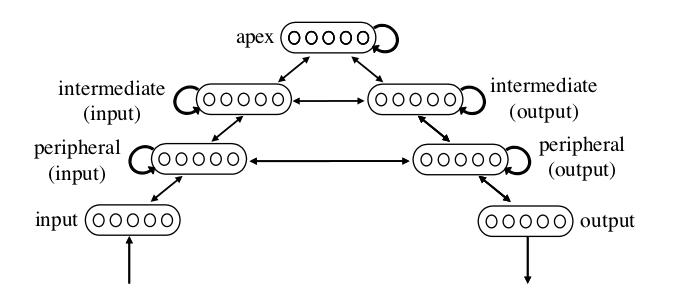
\includegraphics[scale = 0.37]{figures/botvinick.png}
\caption{One of the networks investigated by \citet{Botvinick2007}. When trained on a task with temporal abstraction, the longer timescales were handled by the higher layers. Reproduced from \citet{Botvinick2007}.}
\label{botvinick}
\end{center}
\end{figure}

Very interesting are also the articles by \citet{Dominey1995} and \citet{Hinaut2011}, in fact the first example of reservoir computing and a recent continuation of this line of research. In \citet{Dominey1995} rather elaborate letter sequences are learnt by a recurrent neural network, that has a topology explicitly based on PFC and BG structure. The nodes representing the PFC even have different time constants and it is noted that this increases the robustness of the performance, although any structure in the PFC was not investigated. Reading this article is highly recommended. \citet{Hinaut2011} give a computational account of sequence categorization: as we noted before, abstractions are necessary to deal with large numbers of possibilities, in this case possible sequences. This can be considered relational integration of temporal abstraction. A recurrent neural network with three layers, corresponding to the infragranular, granular and supragranular layer, was trained to repeat presented sequences. The result is that some nodes in the recurrent neural network show sequence categorization, matching measurements from primate PFC.

A model that did not originate from action sequences, but from working memory research is the PBWM (PFC BG Working Memory) model by \citet{Frank2001}. The structure of this model is illustrated in figure \ref{oreilly}. It is based on the reported loops between the PFC and BG (see section \ref{loops}). The topology is quite similar to the one in \citet{Dominey1995}, but the model functions differently: through so-called adaptive gating in which the BG update PFC representations. The model has been shown to solve working memory related tasks and is compared with competing architectures by \citet{O'Reilly2006}. For us, the most interesting study using this model is \citet{Reynolds2009}: they show that tasks can be learned faster when abstraction levels are processed topologically in a hierarchically structured network, compared to a hierarchically structured network in which the abstraction levels are not processed topologically. Note however, that when the PFC network is not structured hierarchically (and abstraction levels are not processed topologically), learning is finished even faster and the performance better.

\begin{figure}[tbhp]
\begin{center}
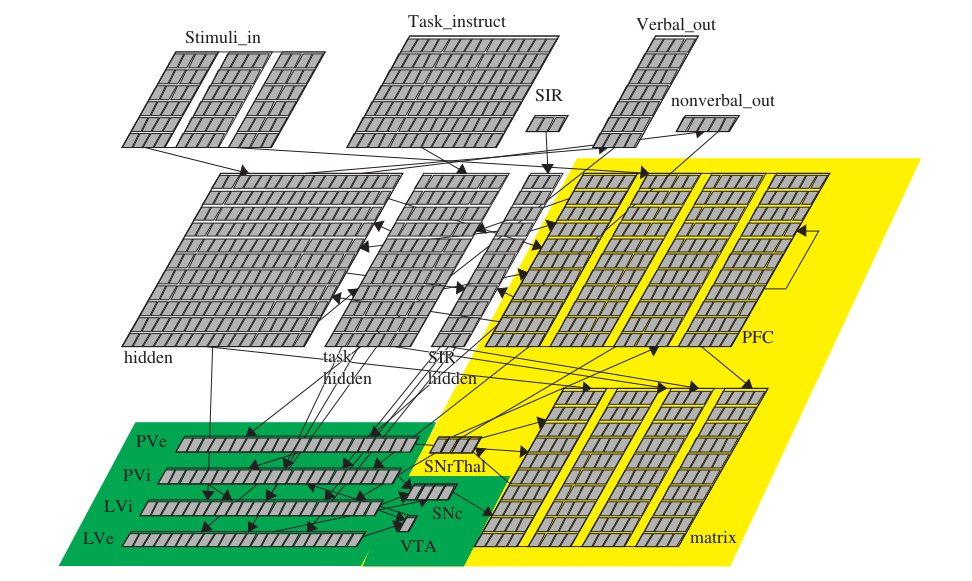
\includegraphics[width=\textwidth]{figures/oreilly.png}
\caption{One (non-hierarchical) version of the biologically plausible PBWM model. Each small rectangle is a neuron and is part of a specific brain network. This system can be trained to perform rather complicated tasks. Reproduced from \citet{Hazy2007}.}
\label{oreilly}
\end{center}
\end{figure}

Finally, we have to mention a small model that was explicitly inspired by \citet{Koechlin2003}. \citet{Koechlin2007} describes how a recurrent neural network inspired by FPC can be used for branching: a temporary lapse from the current episodic context to a new one, to return when the new episode is over. While branching is an interesting idea and a form of temporal abstraction, the model does not seem to prove anything: it is not surprising that a recurrent neural network of slight complexity supports such a task. Perhaps future invasive recordings can validate or invalidate this model though. Anyway, for us this model is not very interesting, because it does not implement lower levels of the hierarchy proposed by \citet{Koechlin2003}.

All in all, with all these different results, we still do not know how the abstractions are different from or similar to each other and why exactly it could be an advantage to map abstraction levels to PFC areas. It could be an advantage for learning, as described in \citet{Reynolds2009}, allowing for faster or easier re-use of policy abstractions or perhaps for input targeted at a specific abstraction level. It could also be an advantage for cognitive control, as described in \citet{Botvinick2007}: higher temporal abstraction levels should not be disturbed by what is going on at lower levels and should therefore be located at a larger distance from input nodes. Or following \citet{Koechlin2003}, high level concepts do not carry any information that can directly be used for the output, and should therefore be located at a larger synaptic distance from the motor areas. Note that these ideas make the implicit assumption that shorter connections are better than longer ones (which is an embodied argument), if they are to explain the evolutionary development of the PFC. 

A problem is that all those models were used to solve artificial tasks, just like the subjects of the imaging experiments. This are not the tasks that have given the brain its structure and may overlook some important insights. Therefore, we also look at robot control systems and models.

\subsection*{Efficient Cognitive Control for Robots}

The advantage that a hierarchical control system has for robots is that it is more efficient than a controller without abstraction \citep{Dijk2011}. Due to the complexity of the real world this efficiency is often even a necessity, explaining the popularity of hybrid robot controllers and adaptive behavioural systems \citep{Scheutz2004}. One idea that had a large influence on the current study is regulative control \citep{Lagarde2010}. This is a subsumption architecture with an adaptive layer that can change which layers are active in a particular situation, implementing policy abstraction. This gives a computational advantage over controllers that do not use abstraction. Apart from regulative control, a number of other studies are relevant for this thesis.

To start with the most important article, \citet{Paine2005} used a CTRNN to show that a small fully connected network is less successful in a maze navigation task than a network with a bottleneck in the middle (with the same number of nodes). The more abstract input of the goal in the maze is given at the top of the network, while sensory input is given at the bottom of the network. This architecture is illustrated in figure \ref{tani}. An EA was used to train the weights of the connections and time constants so that the simulated robot could drive to the desired goal position in the maze. Apart from the performance difference, it was also found that the time constants at the top of the network were larger than the time constants at the bottom of the network. This result does give a possible explanation for the development of a hierarchical structure (although this was not tested directly), but does not explain why the long term input is offered at the top of the network, while the sensory input is given at the bottom of the network. It is also not tested how the bottleneck network would perform if the information was not presented and processed topologically or whether the sparsity of the network influenced the results. \citet{Maniadakis2010} used the same network for robots that can solve a WCS task. 

\begin{figure}[tbhp]
\begin{center}
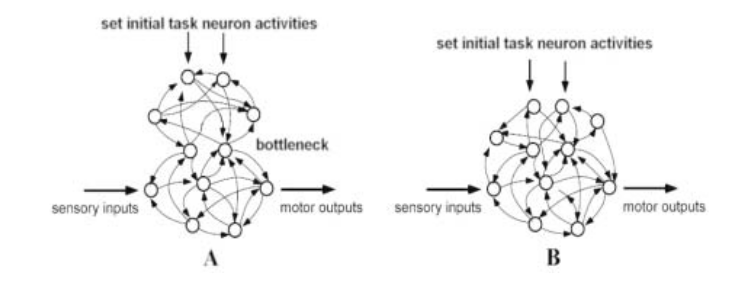
\includegraphics[width=\textwidth]{figures/tani.png}
\caption{The CTRNNs that were investigated by \citet{Paine2005}. Reproduced from \citet{Paine2005}.}
\label{tani}
\end{center}
\end{figure}

The study conducted by \citet{Yamashita2008} resembles the study by \citet{Botvinick2007}, but now a real robot is taught to handle an object. A CTRNN is organized hierarchically by coupling three sections with different time constants: an input-output layer, a fast context layer and a slow context layer. BPTT is used to teach the network the desired joint angles for a number of overlapping action sequences. \citet{Yamashita2008} also show that motor primitives are re-used for the overlapping parts. Unfortunately, again the question of whether or how the hierarchical structure is actually beneficial is left untouched. 

Another interesting robot controller is presented in \citet{Prescott2006}, inspired by BG models like PBWM. Discrete actions are defined as in a behavioural system, but the action selection process is driven by a BG model. The model is tested on real robots doing a couple of tasks, and shown to give good action selection results. While it gives an idea about how a neuroscience model can be implemented and tested in robots, it does not include an account of PFC. Another quite detailed model is presented by \citet*{Khamassi2011} and focuses on ACC and lPFC: an iCub was taught a simple game in which a human could change rewards. Eventually, the robot learned to change its behaviour after human intervention. 

All in all, the number of models of PFC function is considerable, but the number of robot controllers inspired by it is quite small. Although we were not able to create a robot controller ourselves, we would like to keep this application in mind while building our model. We can combine some good ideas from the robot controllers and PFC models described above to do this efficiently. One of those ideas is to use an echo state state network to model PFC, similar to \citet{Dominey1995}. 

\section{Echo State Networks}
As the reader may have noticed, most of the models use either BPTT or RL for training. We chose however to use an ESN because it is computationally cheap compared to other neural network methods and is therefore more suitable for autonomous robots. Thus, reviewing the current state of affairs in ESN research will help us with the construction of our model. As described in the previous chapter, ESNs have been established as a good method for timeseries prediction and also for some classification problems. As ESNs are a reasonably new development, these first applications are still under investigation (see for example \citet{Zhang2012}). However, a couple of other applications and research directions have been investigated as well. We will discuss four developments that are interesting for us.

First of all, quite some effort was spent to attempt to make ESNs work on different time scales. This is important, because our model should work over different time scales (levels of temporal abstraction). Most notably, Jaeger himself wrote one report about discovering features on multiple time scales with a hierarchical architecture \citep{Jaeger2007}, which is illustrated in figure \ref{hierarchicalESN}, and collaborated on a technical report about ESNs that can handle time warping \citep{Lukovsevicius2006}. As far as we are aware, the hierarchical architecture was never applied on more problems than the simple examples described in the technical report, so we can unfortunately not determine how good its performance is. Also, the precise design of the architecture requires closer investigation, according to Jaeger in his conclusion. The ``time warping invariant'' ESNs are made with leaky integrator neurons of which the time constant can globally be adapted to the speed of the input signal. These leaky integrator neurons bring the ESN closer to a CTRNN compared to the discrete time steps that are usually used. In \citet{Jaeger2007a}, ESNs with leaky integrators are used for classification of audio recordings of vowels and the ideas about its advantages and use for time warped signals are discussed (more clearly than in \citet{Lukovsevicius2006}). 

\begin{figure}[bthp]
\begin{center}
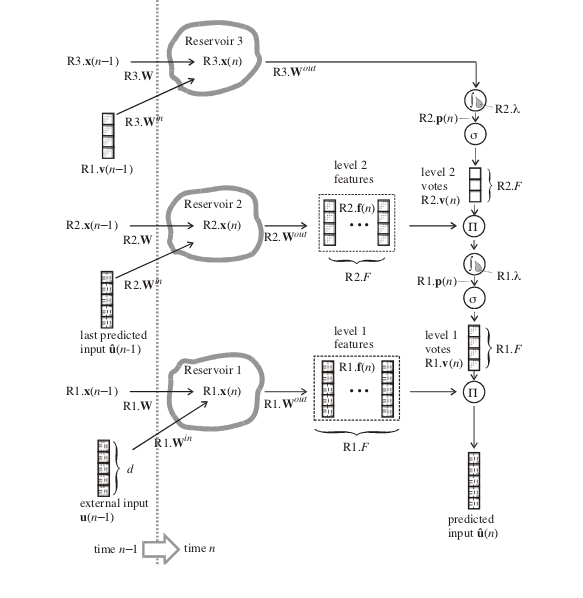
\includegraphics[scale=0.5]{figures/ESNstack.png}
\caption{Three stacked ESNs can discover features on multiple time or spatial scales. Reproduced from \citet{Jaeger2007}.}
\label{hierarchicalESN}
\end{center}
\end{figure}

Secondly, structure in ESNs has received attention as well. We will roughly model the structure of PFC, making this direction relevant. Apart from aforementioned hierarchical system by \citet{Jaeger2007}, \citet{Xue2007} is a good example. Their method is based on a number of separate ESNs and a lateral inhibition system. The different ESNs receive the same input, but the lateral inhibition system assures that the networks process different features. The resulting network gives better performance and better robustness with respect to the exact initialization of the random connection weights. Another study that is worth mentioning is \citet{Jarvis2010}. Here, the ESN was initialized to be more or less clustered and the effect on the echo state property investigated. It was shown that clustered ESNs allow for larger spectral radii to still show the echo state property, while more homogeneous networks required a smaller spectral radius to maintain stability. Other suggestion include altering the connections in the reservoir to improve on the random initialization of the ESN \citep{Sussillo2009,Dutoit2009} and ``scale free highly clustered ESNs'' \citep{Deng2007}. Alse see \citet{Kaiser2010} for a more general study about the relation between network size, modularity and stability.

Thirdly, ESNs have been applied for robot control, as we designed our model for. Apart from applications in which the ESN was responsible for the inverse model of motor actions (e.g., \citet{Ploger2004}), ESNs have also been applied for motor control (e.g. \citet{Salmen2005} and \citet{Morse2009a}, a very interesting combination of ESN and Adaptive Resonance Theory for classification of input patterns). Perhaps the most promising studies to date are \citet{Hartland2007} and \citet{Waegeman2009}. In these studies, ESNs are used for learning by demonstration of motor actions, showing good results. \citet{Waegeman2009} uses a hierarchical ESN: the bottom layer is used to learn the basic goal seeking and obstacle avoidance behaviours, while the top layer afterwards learns to coordinate these two behaviours. Another interesting application can be found in \citet{Antonelo2011}. In this study, the ESN is used to non-linearly process input signals from a robot. The output of the network is then learned by an unsupervised slow feature analysis (SFA). The final result is an autonomous robot localization system, analogous to hippocampal place cells in animals.

Finally, at least one research group has trained the output weights of ESNs by artificial evolution \citep{Jiang2008, Devert2008, Hartland2009}. They found that for a simulated motor control task an evolutionary algorithm can outperform the standard learning procedure under certain conditions. This is an interesting development, as it allows ESNs to be trained unsupervised. A slightly different approach is taken by \cite{Krause2010}: they use an EA to find the optimal settings for the parameters of the reservoir. These studies suggest that the large field of evolutionary neural networks may be extended with ESNs. There might be two advantages compared to other methods (like NEAT for example): because only the output weights have to be learned the algorithm might converge to a good solution quickly \citep{Devert2008} and it can be integrated easily with behavioural robotics. These two advantages might make it a good candidate for online evolution in robots; see the future research section for further elaboration.

The most important points to keep in mind are that standard ESNs do not work well when the task involves multiple timescales and that structure in the ESN may change the properties of the reservoir. This will help us to construct a structured ESN that can handle multiple timescales. With this ESN, we can investigate whether the requirements of information integration and preservation in cognitive control tasks can explain segregation of abstraction levels, as has been measured in the PFC in a number of fMRI studies. 

\chapter{Methods}
In this chapter, we will describe how we used the information from the literature to construct our ESN and define its tasks.

\section{How Brain Structure Can Support Tasks}
As stated in the introduction, we hypothesize that control tasks that involve policy or temporal abstraction both require information preservation between the abstraction levels and information integration within the abstraction levels. We will use an Echo State Network to investigate this claim, as will be detailed in the following sections. However, even if we can confirm this hypothesis, we still have to make the step to mapping of abstraction levels in the prefrontal cortex. Thus, we will present two lines of thought here that make this step plausible: the first argumentation requires the ESN to be a direct model for PFC, the second and main argumentation uses the ESN to confirm our hypothesis and explains how this leads to the mapping of abstractions in the PFC.

If we assume the ESN to be a model for PFC, we have to align the random connections in the ESN with the far from random axon growth in the PFC. This is easier than it may seem: good performances in a random ESN imply that the targeting of axons in the PFC can be relatively inaccurate (closer to random) without endangering its functionality, compared to a situation that corresponds to a weak ESN performance. As a rather large number of axons has to grow in the PFC, less accurate targeting can save effort and resources (time, space, energy and materials \citep{Sporns2010}). Thus, a PFC with a structure that corresponds to the better performing ESN may have a small evolutionary advantage, because it may take slightly less targeting effort in the PFC to obtain the same performance. The weak points of this argument are that it is not certain that the structure in an ESN has the same effect on performance as the structure in PFC and, related, that it is not clear how accurate or inaccurate axon growth is \citep{O'Donnell2009}.

Therefore, our main argumentation does not interpret the ESN as a direct model for PFC; instead, we only use it to support our hypothesis that cognitive control tasks that involve policy or temporal abstraction share the requirement of information preservation between the abstraction levels. Thus, we have to make a second step and answer the question why the PFC can better integrate information within an area and better preserve information by segregating it spatially. It is most likely that for integration of information more connections are required than for keeping information separated. Therefore, the total axon length that is required in the PFC is smallest when information is integrated within each area, and preservation of information is obtained by processing it over different areas. That total axon length is in fact minimized by evolution is known as the wiring economy principle \citep{Allman2000, Cherniak1994, Sporns2010} (note that this is also an excellent example of embodied neuroscience). Thus, if we can confirm our hypothesis, we can also explain the topological mapping of abstractions in the PFC.

\section{Network Architecture}

Echo State Networks do not inherently have the possibility to control the location of processing: the input activity spreads over the whole network. However, to assess the influence of topological processing of abstraction we do want to control the place where information is processed. The solution is to control the way in which input is presented to the network: if we connect all input nodes to all parts of the network, no topological processing will be possible. After all, all input information will already be mixed by overlapping input or otherwise very quickly be mixed due to the random connectivity. If one input node is connected to a different part of the network as the other input nodes however, this can lead to a degree of topological processing. The two input methods are illustrated in figure  \ref{ESNarchitecture}.

\begin{figure}[bthp]
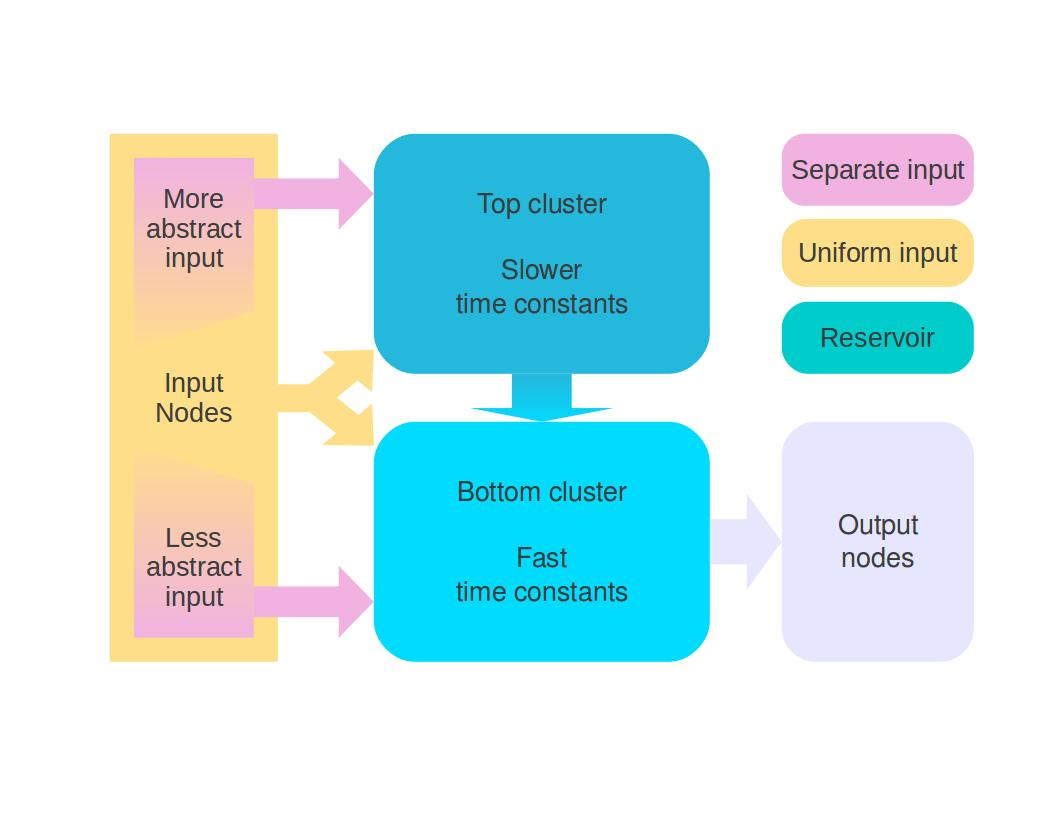
\includegraphics[width=\textwidth]{figures/reservoir1.jpg}
\caption{The architecture of the Echo State Network. In pink and yellow the two input methods, seperated and uniform respectively. In blue the hierarchical topology fashioned after the Prefrontal Cortex. Apart from the constraint on the topology, the connectivity is random. In grey the output nodes for which the weights are trained.}
\label{ESNarchitecture}
\end{figure}

To ensure that coupling input nodes to different parts of the reservoir in fact leads to topological processing, we divided the reservoir of the ESN in two clusters: a `top' cluster and a `bottom' cluster. To enhance the information preservation in the top part of the ESN, we removed the connections from the bottom to the top part of the network, while the information preservation in the bottom part of the network was enhanced by tuning down the strength of the random connections from the top to the bottom part of the network. The random connectivity in each cluster was left untouched, to ensure the information integration capability within each cluster. What is left is a 'top' cluster that influences the 'bottom' cluster but does not receive connections from it. As may be clear already, in the case of separated input nodes, the more abstract node was coupled with the top part of the network while the other nodes were coupled with the bottom part of the network. The activities of the bottom part of the reservoir were used to train the output nodes. This creates a hierarchy as proposed by \citet{Koechlin2007}. When the identification and processing of input is seen as a process separate from top-down control and action selection, this architecture is also compatible with other models, for example those proposed by \citet{Botvinick2007} and \citet{Fuster2002}. 

Special attention has to be paid to the time constants (or leaking rates) in the reservoir. As the output changes on the timescale of one trial (which means one input pattern and a fixed number of timesteps), the time constants in the bottom part of the reservoir have to be fast. The time constants in the top part of the network do not have this restriction and are initialized to a broad range of values that supported the timescale of the task at hand. Thus, for investigating policy abstraction, the top and bottom part of the network covered the same range of time constants, while the time constants of the top part were slower when investigating temporal abstraction (both for the uniform and the separated input connections). Note that this introduces yet another aspect in the hierarchy of the ESN in the tasks involving temporal abstraction. Different settings of time constants were investigated to obtain the best overall performance; note that the resulting differences in performances between the input methods were unaffected.

\section{Tasks}

In the previous sections, we described the structure of the ESNs we will use and that we would like to find performance differences between an ESN with separated input and an ESN with uniform input. These performance differences will tell us whether information integration and preservation is a factor in cognitive control tasks that involve abstractions, as we hypothesized. Thus, it is of importance that we clearly define such tasks. Because we would like to explain the imaging results, our tasks are inspired by and very similar to the tasks that subjects were required to do in the fMRI scanner. We chose the two most studied abstraction types: temporal abstraction and policy abstraction.

\subsection*{Abstractionless Task}
A simple abstractionless task was chosen to give a baseline for the ESN performance and to serve as a basis for the abstract tasks. In good psychometric tradition, the tasks consisted of a number of trials and the task performance was measured as the number of correct responses divided by the total number of trials. At the first time step of each trials, an input pattern was presented to the artificial neural network. Using a look-up table, the input pattern uniquely determines the desired output. After a fixed number of time steps, the output of the network was determined by a simple winner-takes-all comparison between the activation of the output nodes. If the most active output node corresponded to the desired output, the response was correct; in all other cases the response was labelled incorrect. At the next time step, the next column of the design matrix was used to initiate the next trial. Note that the network activities were not reset between the trials. 

A real-world example of this task is a classification problem with a small number of binary inputs. A robot could for example classify the current context each second by using the amount of light in the environment (day or night), the battery status (empty or full) and the acoustic conditions (silent or just heard some noise). This classification could then be used to select the behaviours that are most appropriate in each context, for example a ``find out what happened''-behaviour when it is night, the battery is full and the robot just heard some noise.

\begin{figure}[bthp]
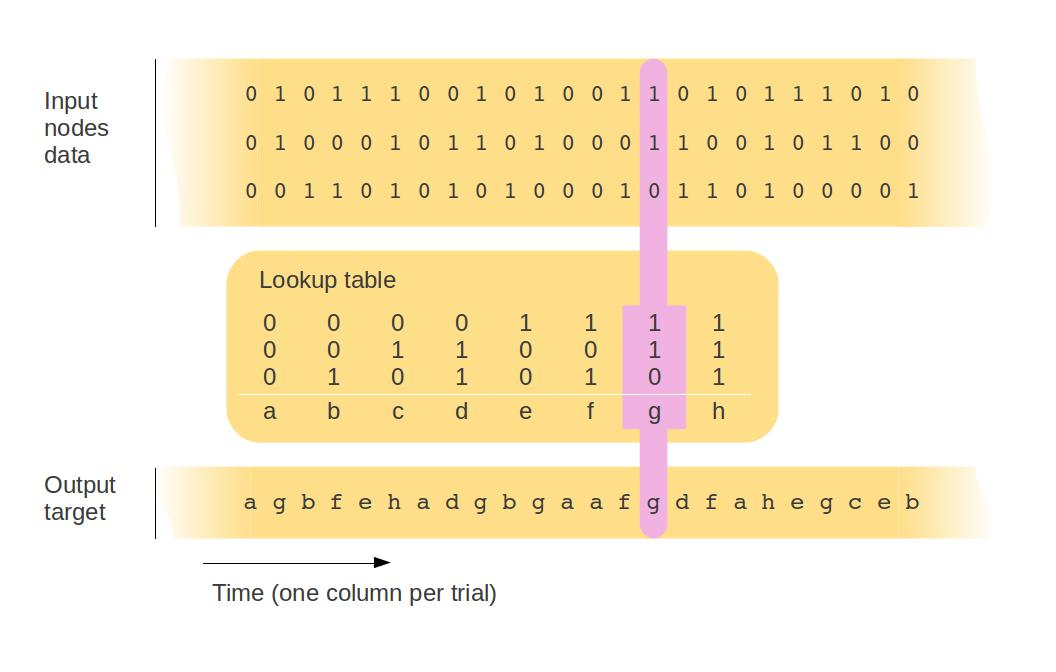
\includegraphics[width=\textwidth]{figures/tasknoabstr.jpg}
\caption{A simple task without abstraction that is used as the basis for the tasks in the simulation. At each trial, each input node assumes either a high state or a low state. The sequence of these input patterns over all the trials is stored in the design matrix. A look-up table is used to determine which output node is associated with a specific input pattern. }
\label{abstractionless}
\end{figure}

\subsection*{Temporal Abstraction}
The task without abstraction is readily extended to a task with temporal abstraction: one input node is selected to be more abstract than the other nodes and the node's row in the design matrix is subsequently moved a certain number of trials towards the past. This is illustrated in figure \ref{temporal}. The result is that the current value of this node has to be used to find the correct output a certain number of trials in the future, instead of finding the currently expected output. To solve the task, the ESN therefore has to ``remember'' the input values for a certain period, quite similar to a person doing an n-back test. 

The most obvious case of this task happening in real robots is when some perceptions are processed faster than others. In this case, information with a small time difference has to be integrated. For example, it may be obvious immediately whether it is day or night, but it may take a while before it is clear whether anybody is coming in your direction on the street using either vision or sound. Then, the robot should remember for a short time whether it was light or dark at a certain moment and then integrate this with the information that is coming in later. Longer time spans may also be required, for example when the robot somehow receives a message that means ``pay attention for the next ten minutes''.

The condition that will be varied in this task is the length of the temporal abstraction. If our hypothesis is correct, and separating abstraction levels in this task helps by preserving information, the ESN with separated input connections should have a benefit when the task covers a longer timespan. Reversely, when the task is easier, such as a 1-back task, preservation of information is less important than integration of information and the ESN with uniform input should have an advantage. Note that a result in which the performance of one of the input methods is better in all conditions is not useful: how much better it is may depend on our performance metric instead of the difference in the task conditions. Thus, merely comparing the performance differences cannot confirm our hypothesis if all these differences are either negative or positive. Instead, we need a change in the sign of the differences over the range of conditions.

\begin{figure}[bthp]
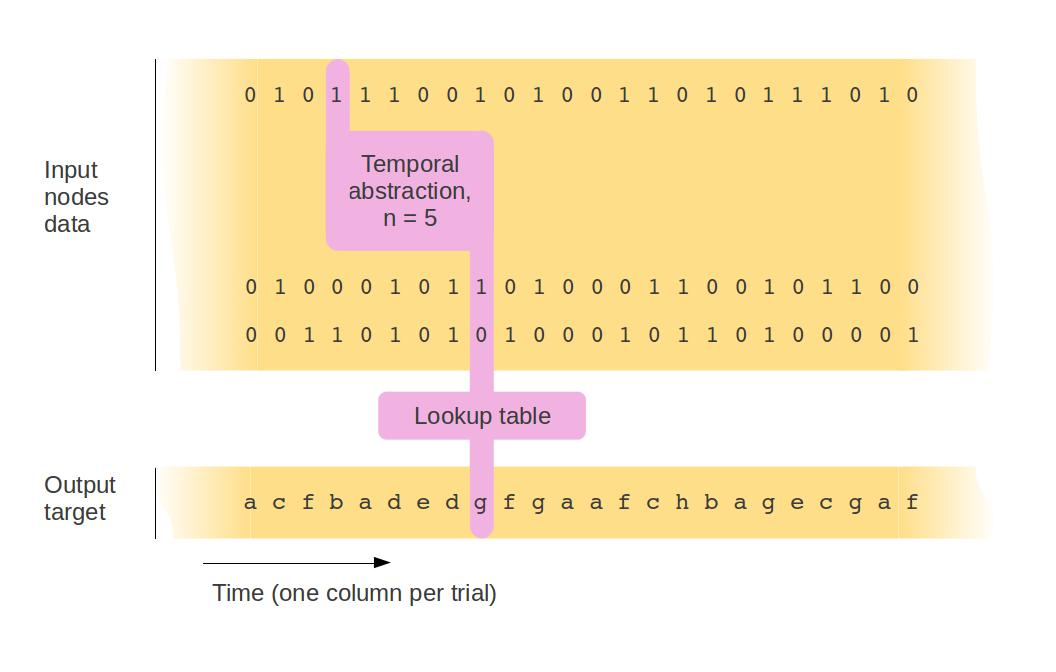
\includegraphics[width=\textwidth]{figures/tasktemp.jpg}
\caption{The implementation of the temporal abstraction used in the simulations. The design matrix and output matrix are built using the task without abstraction described before. The temporal abstraction is then achieved by presenting the relevant bit from one of the input nodes a number of trials earlier than the data at the other input nodes. In the figure a delay of five trials is shown. Thus, each trial one column of the design matrix is presented, but to obtain the desired output, the bit that was presented at the first output node five trials ago has to be used instead of the bit that is presented at the first node currently. This design leads to a chance level of 50 percent when the bit from the first input node could not be remembered, while the other input bits could be successfully integrated.}
\label{temporal}
\end{figure}

\subsection*{Policy Abstraction}

%is generalization unsupervised policy abstraction???!!!

To obtain a task with policy abstraction, a slightly larger change has to be made. Instead of coupling each input pattern uniquely with one output node, we now allow ourselves to couple input patterns that are partly the same with one output node. This way, we can choose one input node that is important for all of the trials and is more abstract, while the other input nodes are only important in half of the trials and are less abstract. Which set of input nodes is important for the current trial is then of course determined by the abstract input node. This is similar to the sorting part of the \gls{wcs} task: we have to base our sorting or classification on only part of the cues we get, while the rest of the cues are mere distractors. Alternatively, a more computer science-minded person may prefer to understand this task by noting that the distractors can be implemented by using wildcards in the look-up table. The task is illustrated in figure \ref{context}.

A real-world example of this task could be crossing a street. If it is day (input one, the context), the most accurate information will be visible input. If the robot can see something big heading its way (input two, the relevant cue), it should not cross the street. If it is night on the other hand (different context input), the most important information is audio input. If the robot can hear somebody coming (input 3), it should not cross the street, ignoring any unreliable visual information (input two is now a distractor).

The condition that will be varied in this task is the number of low-level cues that are presented (and therefore also the number of output nodes). If our hypothesis is correct, and separating abstraction levels in this task helps by preserving the more abstract information, the ESN with separate inputs should have an advantage on tasks with a large number of low-level cues. When only a small number of low-level cues has to be integrated, the preservation of the high-level cue is not very important and the ESN with uniform input should perform better. Again, only by showing that the performance difference changes sign when comparing the conditions with a small number of low-level input nodes with the conditions with a large number of input nodes, we can confirm our hypothesis.

\begin{figure}[bthp]
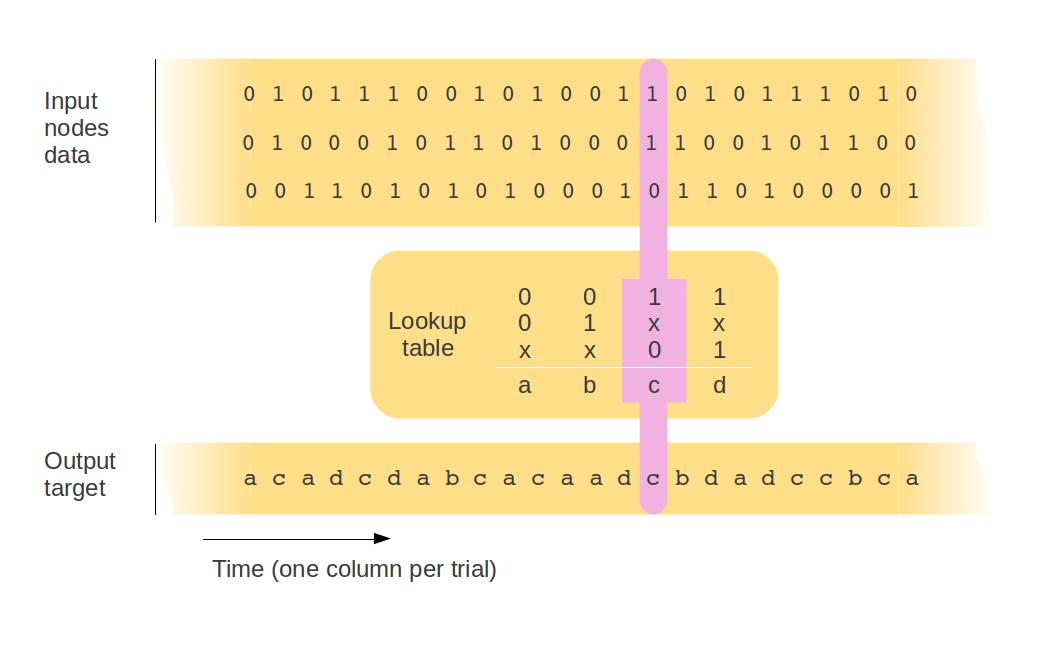
\includegraphics[width=\textwidth]{figures/taskpol.jpg}
\caption{The easiest version of the policy abstraction task used in the simulations. The x in the lookup table is a wildcard: the input can be either high or low, it is irrelevant for the task and thus a distractor. The number of outputs for this task equals $2^{n+1} $ with $ n $ the number of low level cues per context. This brings chance level to 50 percent when the abstract cue cannot be integrated with the rest of the cues, and to $2^{-(n+1)} $ when none of the cues can be integrated due to the distractors.  }
\label{context}
\end{figure}

\section{Learning}

Now that we know the architecture of the network and the task, we can describe how the network will learn the task. As with most applications of ESNs so far, we will use linear regression. Let $\vec{d}$ be the vector with the successive desired values of one output node and let $S$ be the state collection matrix: a matrix in which each row is filled with the state of the reservoir at the successive trials. Then we have to find the best solution to the following equation:
\[  \vec{d} = S \vec{w} + \epsilon \]
With $\vec{w}$ the output weights for this node and $\epsilon$ the error. The method we use to solve this is by minimizing the sum of squares of $\epsilon$, which is linear regression and can be done with the following equation:
\[ \vec{w} =  S \sp{\dagger} \vec{d} \]
With the dagger denoting the pseudoinverse. Obviously, this can be extended to multiple output units and a weight matrix. While this method was sufficient and effective for our current application, better performances may be obtained by using more sophisticated regression methods. Regularization for example may reduce the effect of uncommon distractors by favouring smaller weights. A simple way to do this would be to use ridge regression instead of linear regression \citep{Jaeger2007b}. Also note that linear regression procedures are more suitable for timeseries prediction than for the binary classification problem we try to solve; therefore, logistic regression might also give a significant improvement.

\section{Network Dynamics}

While the dynamics of the reservoir can in principle be arbitrary, choosing a good reservoir for the task can make the difference between performance at chance level and performance that rivals state of the art methods. Here we discuss three choices that concern the dynamics in our reservoir: the use of time constants or leaking rates, the activation function, and the way the input is added to the network activation.

\subsection*{Continuous Time Echo State Network}

The first ESNs were recurrent neural networks in discrete time, with updating steps according to equation \ref{update}. This method works perfectly for timeseries prediction when only one timescale is of importance and the output depends critically on inputs at very specific points in time. However, for classification problems, the specific point in time of a feature may vary, leading to the introduction of ESNs with leaky integrator neurons \citep{Jaeger2007a}. These are more capable of dealing with small variations in timing and have been shown to perform very well on a vowel classification task, using the following updating equation:
\begin{equation}
 \vec{A}_{\text{new}} = (1 - a) \, \vec{A}_{\text{old}} + f(W \, \vec{A}_{\text{old}} + \vec{u} + \vec{b} ) 
 \label{leaky}
\end{equation}
With $a$ the so-called ``leaking rate'', which is constant for the whole network, and $\vec{u}$ the input to each node, which is calculated using an input weight matrix. In practice, the leaking rate is chosen to be rather large, between 0.1 and 1 (which corresponds to a discrete time ESN). When we compare this to the updating equation (using Euler integration and $\Delta t = 1$ ) for Continuous Time Recurrent Neural Network (CTRNN), we note a striking similarity:
\begin{equation}
 \vec{A}_{\text{new}} = (1 - \frac{1}{\tau}) \, \vec{A}_{\text{old}} + \frac{1}{\tau} \, (W \, f(\vec{A}_{\text{old}} + \vec{b} )  + \vec{u} ) 
 \label{ctrnn}
\end{equation}
Obviously, this approximation of continuous time is only reasonable if the time constants $\tau$ are large enough; a general rule of thumb is that they should be larger than ten times $\Delta t$, which comes down to larger than ten in the formula above. Thus, apart from the different order of applying the activation function and the weight matrix, the leaky ESN corresponds to a coarsely integrated CTRNN.

Of course, we now have to find an answer to the question how we should define our own updating equation. For this choice, the most restricting aspect of our tasks is that it should be possible to cover multiple timescales. Also, we would like to achieve tolerance for timing differences and noise. Discrete time ESNs are thus not the ideal solution for our network. Although it would be possible to introduce different timescales by using different sampling rates, or by creating a hierarchy of reservoirs as \citet{Jaeger2007} did, timing differences will probably still cause problems. Therefore, we turn to leaky integrator ESNs. However, a critical disadvantage of this solution is that the leaking rate is fixed for the whole network. While in principal it is possible to create a semi-discrete time network with different leaking rates, in practice this solution turns out to be not very effective (according to \citet{Jaeger2007a} and our own observations). This is probably caused by the fact that the approximation to continuous time is insufficient.

Thus, we will use a leaky integrator ESN with very small leaking rates to approximate continuous time better than usual leaky integrator ESNs. As this corresponds so well with the existing CTRNN equations, we decided to explicitly match our update equation to them with respect to the time constant, yielding a Continuous Time ESN (CTESN): 
\[  \vec{c} = \frac{1}{\tau} \]
\[  c_i \leq 0.1 \]
\begin{equation}
 \vec{A}_{\text{new}} = (1 - \vec{c} ) \, \vec{A}_{\text{old}} + \vec{u} + \vec{c} \, f(W \, \vec{A}_{\text{old}} + \vec{b} ) 
 \label{ourupdate}
\end{equation}
Again, with the operations working elementwise. The reason that the input is added directly to the activation is discussed in the subsection ``input method''. This formula leads to a more well-behaved and transparent handling of multiple timescales, also increasing the performance in some circumstances. Also, we maintain at least the biological basis of the neural network instead of making a purely abstract model with a standard ESN. However, we also have to accept two downsides: the amount of computation is multiplied about tenfold, and in tasks that have a single timescale, performance is greatly reduced compared to a leaky integrator ESN with a leaking rate tuned to the problem.

The updating equation for the CTESN has some interesting influences on the dynamics of the reservoir as well. The standard ESN dynamics are best understood by examining an ESN with a linear activation function. Each time an input is given, it is stored in the network in a specific scale and pattern depending on the input weights. At the next timestep, these values are stored in another pattern and slightly scaled down (because the spectral radius of $W$ is smaller than one). This way, each input over the past timesteps is retrievable by the output layer. When we change the activation function to be a tanh, the principle is exactly the same, except that large values are not stored linearly, making non-linear behaviour possible. However, as you may have noticed, these dynamics are dependent on the coarse euler integration of the network: only because of this coarse integration it is the spectral radius that determines the duration of the echoes. Without this overshoot the network returns to the fixed point much faster and input separability quickly becomes very small. 

This explains the reduced performance in CTESNs and leads us to the question how CTESNs can perform at all. The answer is that the information is stored in the slowly changing activation value of specific nodes, instead of in a fast changing pattern \citep{Schrauwen2007}. Clearly, this is also the reason that small differences in timing of input signals do not degrade the performance very much: the difference in activation will be small. Also, this brings to light another advantage of CTESNs over other types of ESN: the memory length is not limited by the reservoir size but only by the leaking rates of the nodes that are included in the reservoir. To conclude this discussion, an overview of different ESN types is given in table \ref{esncomparison}.

\begin{table}[!h]
\begin{center}
  \begin{tabular}{ | p{2.1cm} | p{2.8cm} | p{2.8cm} | p{2.8cm} | }
    \hline
    ESN & Discrete Time & Leaky Integrator & Continuous Time \\ \hline \hline
    Storage & Fast changing patterns & Patterns and activations & Slowly changing activations \\ \hline
    Tasks  & Timeseries prediction & Vowel classification & Action sequences, context classification? \\ \hline
    Input Timing & Critical & Intermediate & Relaxed \\ \hline
    Input seperability & Good & Intermediate & Poor \\ \hline
    Timescale & Determined by sampling rate & Sampling rate and tunable by leaking rate & Multiple \\ \hline 
    Computational Cost & Low & Intermediate & High \\ \hline
    Memory Length & Limited by reservoir size & Limited by reservoir size & Limited by leaking rates \\ \hline   
  \end{tabular}
\end{center}
\caption{The differences between discrete time, leaky integrator and continuous time ESNs.}
\label{esncomparison}
\end{table}


\subsection*{Activation Function}
In the updating equation \ref{ourupdate}, the activation function is left unspecified. Two common choices for the activation function of nodes in recurrent neural networks are the tanh and the sigmoid (more specifically, the logistic function). The difference between those two activation functions is interesting, as the formulae are quite similar. The difference that is important in the ESN setting is that logistic nodes give 0.5 output when no input is present, while the tanh nodes give 0 output in that situation. That means that the stable fixed point without input is just the zero state in case of tanh nodes, while this is not the case for sigmoid nodes: due to the nodes giving some output, some nodes will have a higher `base' activation than others depending on the input weights of each node. The result is that sigmoid nodes have a built-in bias, which can result in richer dynamics of the ESN. Indeed, random biases are often added to tanh networks to achieve the same richer dynamics (Vytenis Sakenas, personal communication, February 27, 2012).

The obvious question is whether the logistic and tanh activation functions actually have different dynamics. To answer this question we will construct two networks that have a corresponding activation to begin with and calculate the activation at the next timestep. First we have to look up some definitions; the well-known relation between the tanh function and the logistic function is:
\[ \tanh(x) = 2 \mathrm{G}(2x) - 1 \]
with
\[ \mathrm{G}(u) = \frac{1}{1 + \exp(-u)} \]
the logistic function.

This relation is not hard to derive yourself:
\begin{align*}
 \tanh(x) &\equiv \frac{\exp(x) - \exp(-x) }{\exp(x) + \exp(-x)} = \frac{1 - \exp(-2x)}{1 + \exp(-2x)}\\
  &  = \frac{2 - 1 - \exp(-2x)}{1 + \exp(-2x)} = \frac{2}{\exp(-2x) + 1} - 1 \\
  &= 2 \mathrm{G}(2x) - 1  
\end{align*}

Now suppose that at a certain time the activation vectors of the tanh and sigmoid networks are given by
\begin{equation}
\vec{A}_{\text{tanh}} = 2 \vec{A}_{\text{sigm}} - \vec{I} \label{transform}
\end{equation}
This is possible because the ranges of activation are $ (-1 , 1)  $ and $ (0 , 1) $ respectively. If we can show that the activation in the networks at the next timestep fulfil the same relation, it means that the dynamics of the networks are equal. So, we will calculate the activation vector at the next timestep (labelled "new") for the tanh network using the updating equation \ref{update} and try to express it in the new activation vector of the logistic network. (In this derivation the function of a vector is meant to work on each element of the vector separately, resulting in a vector again. Imagine an index if this is not to your taste.)
\begin{align*}
 \vec{A}_{\text{tanh}}^{\text{new}} &= \tanh(\vec{A}_{\text{tanh}} W_{\text{tanh}} + \vec{b}_{\text{tanh}} ) \\
 &= \tanh( ( 2 \vec{A}_{\text{sigm}} - \vec{I} ) W_{\text{tanh}} + \vec{b}_{\text{tanh}} )   \\
 &= \tanh( 2 \vec{A}_{\text{sigm}} W_{\text{tanh}} - \vec{I} W_{\text{tanh}} + \vec{b}_{\text{tanh}} )  
\end{align*}
Now, set the weight matrices and biases according to:

\begin{equation}
W_{\text{tanh}} = W_{\text{sigm}} / 4 \label{weights} 
\end{equation}
\begin{equation}
\vec{b}_{\text{tanh}} = \vec{b}_{\text{sigm}} / 2 + \vec{I} W_{\text{tanh}} \label{biases}
\end{equation}

then
\begin{align*}
 \vec{A}_{\text{tanh}}^{\text{new}} &= \tanh( \vec{A}_{\text{sigm}} W_{\text{sigm}} / 2 - \vec{I} W_{\text{tanh}} + \vec{b}_{\text{sigm}} / 2 + \vec{I} W_{\text{tanh}} )  \\
 &= \tanh( \vec{A}_{\text{sigm}} W_{\text{sigm}} / 2 + \vec{b}_{\text{sigm}} / 2 )   \\
 &= 2 \mathrm{G}( \vec{A}_{\text{sigm}} W_{\text{sigm}} + \vec{b}_{\text{sigm}} ) - \vec{I} \\
 &= 2 \vec{A}_{\text{sigm}}^{\text{new}} - \vec{I}  
\end{align*}

Thus, if we set the biases and weight matrices according to equations \ref{weights} and \ref{biases} the networks are equivalent. To achieve the same output we can just use the linear transformation given in equation \ref{transform}. As the input in a standard ESN is added to the input in the activation function, the input should be a factor two larger when using the sigmoid activation function as well (another way to look at this is to consider the input to be a temporary change in the bias of a node). Also note that this equivalence is not limited to ESNs; for example, along the same lines, it is possible to show the relation between CTRNNs with logistic and tanh activation functions.  

The decision which activation function to use might seem unimportant now, as the activation functions have been shown to be equivalent. However, the tanh activation function has an advantage: if the biases are set to zero, the network has a fixed point at the zero state. The logistic network without biases on the other hand has a fixed point depending on the weight matrix. If we want it to be the zero state, we require specific biases. Interestingly, \citet{Beer1995} referred to this bias setting as the "zero crossing" of a CTRNN and explains why it is useful . However, the "zero crossing" in a tanh network is much more transparent as it is not dependent on the weights. Therefore, manipulating the weights and biases in a tanh network leads to a more predictable change in network dynamics. This is desirable, especially when constructing reservoirs. Thus, we will use the tanh activation function.

\subsection*{Input Method} 

Finally, we have to choose how the input patterns are presented to the network: the weighted input values can be added to the input of the activation function, as it is done in most ESNs (see equation \ref{leaky}), or the weighted input values can be directly added to the activation level of the node, as we do in equation \ref{ourupdate}. The main reason for this choice is that the reservoir will have a range of time constants. These time constants influence the short term effect that the value of the activation function has, because those two factors are multiplied and then added to the old activation value. Thus, an input that is added under the activation function for a fixed number of timesteps has much less influence on a node with a small time constant than one a node with a large time constant. If the input is added to the activation of the node straight away on the other hand, we do not suffer from this attenuation, increasing the input separability. 

Influencing the activation of the nodes directly has the additional benefit that the effect of the input weights is larger and more direct. This means we can increase the differences in activation levels in the network by increasing the input weights. The result is that the output weights can be smaller. This is an advantage, because ESNs often utilize small changes in the network dynamics, which can lead to very large weights (of the order of $10^{5}$ and up) if the differences in activation levels are small. Such large differences in weight values can give problems when using regularization or evolutionary algorithms when training the weights. The disadvantage of adding the input directly to the activation value is that one step of non-linearity is lost. This should not give large negative effects though, as the number of timesteps per trial is large enough (more than ten). 

Note that a related choice, whether to apply the activation function to the weighted sum of node activations or to take the weighted sum of activation functions applied to node activations, was not investigated. However, this should not make a large difference in dynamics, as this only changes the quantity that is stored in the nodes (at least, as long as the input and output methods are changed accordingly). 

\section{Assessing ESN Activity} 

Having described the dynamics of the reservoir, it is important to find out how the ESN is behaving in practice and what are proper settings for parameters, such as the input scaling. This parameter tuning has always been a challenge in ESN research and is a matter of experience according to \citet{Jaeger2001}. The researchers involved in this project have only limited experience with ESNs, and to make the situation worse, no precedent for classification of binary patterns is known to us. Therefore, we tried to gain some insight in the activity of the ESN with different visualization techniques.

The most obvious and foolproof method of investigating the ESN activity is to plot the activation of a number of nodes at all timepoints in a diagram as in figure \ref{activations}. This immediately reveals the diversity or richness in the reservoir resulting from the input. Of course, one should use the same inputs as in the actual task that has to be solved, as the reservoir activity is not only dependent on the reservoir properties (connectivity, spectral radius, etcetera) but also on the input signals. This overview is useful for determining whether the chosen parameters are in the right ballpark and if not, what is wrong.

Because we decided to use continuous time instead of discrete time, we have the interesting possibility of gaining insight from multidimensional scaling (MDS). MDS can be used to represent high-dimensional data in a lower number of dimensions, usually two or three for easy visualization. This is done by calculating at each point in time how far the current state is removed from all other states using an arbitrary metric. This set of distances is then converted into a low-dimensional set of coordinates. For an review of MDS and similar techniques, see \citet{Borg2005}. When using this method on a standard ESN with a regular task (e.g. NARMA), one would not be able to make sense of the result: every state is different from the other because of the echoes that are still active and the discrete steps in time. That means the result would look like a plate of spaghetti or a cloud of points. However, if we have a discrete set of input patterns and the echoes are not causing big differences in activation patterns, the result of MDS should clearly visualize the effect of the different input patterns in the reservoir. 

The consequence is that the MDS result will look differently for networks that do not have echoes, networks that have weak or normal echoes and networks that are almost independent of the current input and/or exhibit chaotic behaviour. These differences can be seen in figure \ref{MDS}. Although this use of MDS is most useful for an ESN that is used to classify a restricted set of input patters, it might also be possible to assess ESNs with it in general, because it gives a visual representation of the echo state property and the network dynamics. However, as noted before, the performance of a network is also dependent on the specific input properties, so care has to be taken when using this method to assess ESNs designed for solving tasks that take input from an unrestricted set. Moreover, as stated before, this method is not expected to deliver very good results in discrete time. Finally, it may not be possible to directly predict the performance of an ESN with this method; it merely assesses the dominant dynamics. An interesting application of this method might be to find an appropriate spectral radius. We used this method mainly to find proper settings for the bias and input scaling.

\begin{figure}[bthp]
\begin{center}
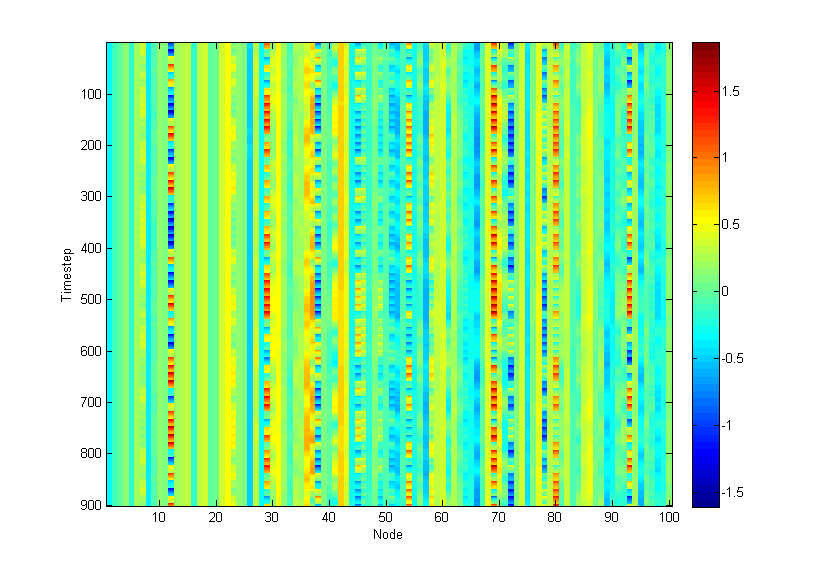
\includegraphics[width=\textwidth]{figures/activations.png}
\caption{An activation plot over 900 timesteps, corresponding to 60 trials. The activation at a number of nodes is almost completely determined by the input: find the repeating red and blue lines. Most other nodes show much fainter activity, which is a non-linear combination of the current and past inputs. }
\label{activations}
\end{center} 
\end{figure}

\begin{figure}
        \begin{subfigure}[b]{0.5\textwidth}
                \centering
                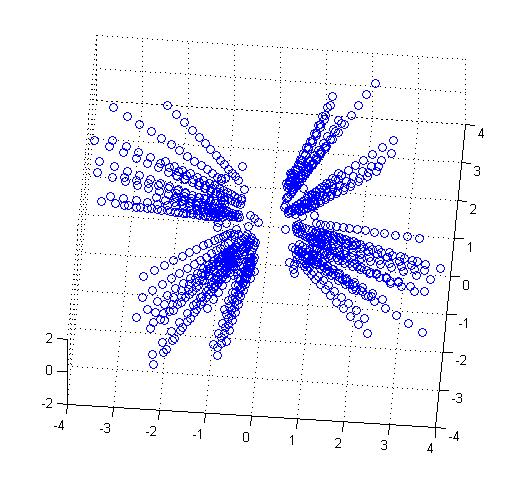
\includegraphics[width=\textwidth]{figures/contraction.png}
                \caption{}
        \end{subfigure}
        \begin{subfigure}[b]{0.5\textwidth}
                \centering
                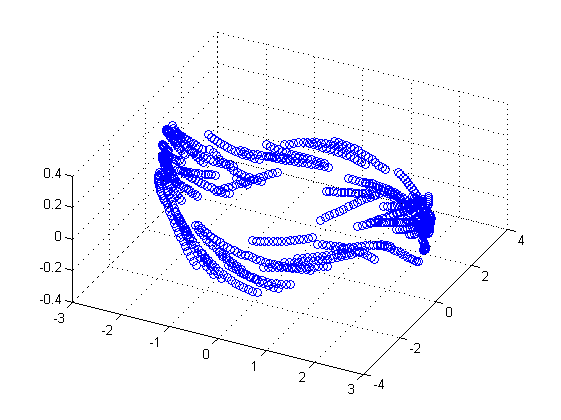
\includegraphics[width=\textwidth]{figures/largeRsmallISsmallB.png}
                \caption{}
        \end{subfigure}
        \caption{MDS plots of ESN activity over 60 trials, with arbitrary units. In figure (a), the activity in the network is dominated by the input patterns: each trials starts at one of the markers that have the largest distance from the origin. Then, thanks to the spectral radius being smaller than one, the activity contracts to the origin of the MDS plot (which corresponds to a stable fixed point in this case). On closer examination, it is possible to find four groups of traces. Each group corresponds to a specific state of two of the three input nodes in the trial (and eight groups could be detected if it would have been possible to print this figure in 3d). The small differences in starting and ending points in each of these groups represent the echo from previous trials, explaining the capability of this network to solve the memory task. In figure (b), the activity of the network is dominated by the internal connectivity, due to a spectral radius larger than one (it was set to two, to be precise). In this case, this leads to a limit cycle with small perturbations by the input patterns. In other networks, a variety of other dynamics could be observed as well. It should come as no surprise that for this network, the test error was much larger than the training error. Nevertheless, it performed well above chance level at a 2-back task; apparently at least some information from the input patterns was stored long enough.}
\label{MDS}
\end{figure}


\section{Implementation}
Most critical aspects of the ESN have been discussed in the previous sections. The architecture, tasks, learning procedure and reservoir dynamics have been defined. Here we will list the parameters that have been used for obtaining the results and address the remaining odds and ends.

An input pattern, consisting of values of -0.5 and 0.5, was presented at the beginning of each trial for the duration of one timestep, with the top cluster of the reservoir receiving the input at the first timestep and the bottom cluster receiving the input at the second timestep. This was done to ensure that the separating the inputs did not have any effects due to the combination of information at a different point in time, although it eventually turned out not to influence the results. After a fixed number of timesteps the activation of each node in the bottom cluster was used for finding the output value. The output node with the highest activation value was the selected output, according to the winner-takes-all principle. Of course, if this node corresponded to the desired output, the trial was counted as correct, and incorrect otherwise.

No washout periods were used between training and testing periods (contrary to other ESN studies) and the reservoir was initialized without any activation. For the regression procedure, a desired output was set to 5, while all other, undesired output node targets were set to 0. For the range of leaking rates, the following formula was used, with $n$ being the memory length:
\[ t = 0.08 \, \exp(-0.2 \, n) \]
\[ \vec{c} \sim U(t , t + 0.02) \]
All parameter settings can be found in table \ref{parameters} and the Matlab code can be obtained from the author and from \url{https://github.com/RemcoTukker/PFC-ESN}.

\begin{table}[!h]
\begin{center}
  \begin{tabular}{ | l | r | }
    \hline
    Property & Value (temporal / policy abstraction) \\ \hline \hline
    Number of Nodes & 100 / 200 \\  \hline
    Number of Nodes Top : Bottom & 1 : 3 \\  \hline    
    Reservoir Connectivity & 0.05 \\ \hline
    Reservoir Weight Distribution & Uniform, centered at 0 \\
    & (but top-down weights are scaled \\ 
    & and bottom-up connections removed) \\ \hline    
    Top Down Scaling & 1.0 / 0.6 \\  \hline
    Spectral Radius & 0.9 \\ \hline
    Input Connectivity & 0.1 \\ \hline
    Input Weight Distribution & $U(-2.5 , 2.5)$ \\ \hline
    Bias Distribution & $N(0 , 0.3)$  \\ \hline
    Timesteps Per Trial & 15 \\ \hline
    Number of Training Trials & 800 \\ \hline
    Number of Test Trials & 800 \\ \hline
    c (leaking rates) & $\pm$0.0001 to 0.1 / 0.08 to 0.1 \\ \hline
  \end{tabular}
\end{center}
\caption{The parameter settings of the ESNs. Note that weight scaling in the reservoir is determined by the spectral radius and the random connectivity; no fixed values can therefore be given.}
\label{parameters}
\end{table}


\chapter{Results and Discussion}

\section{Results}

\begin{figure}[bthp]
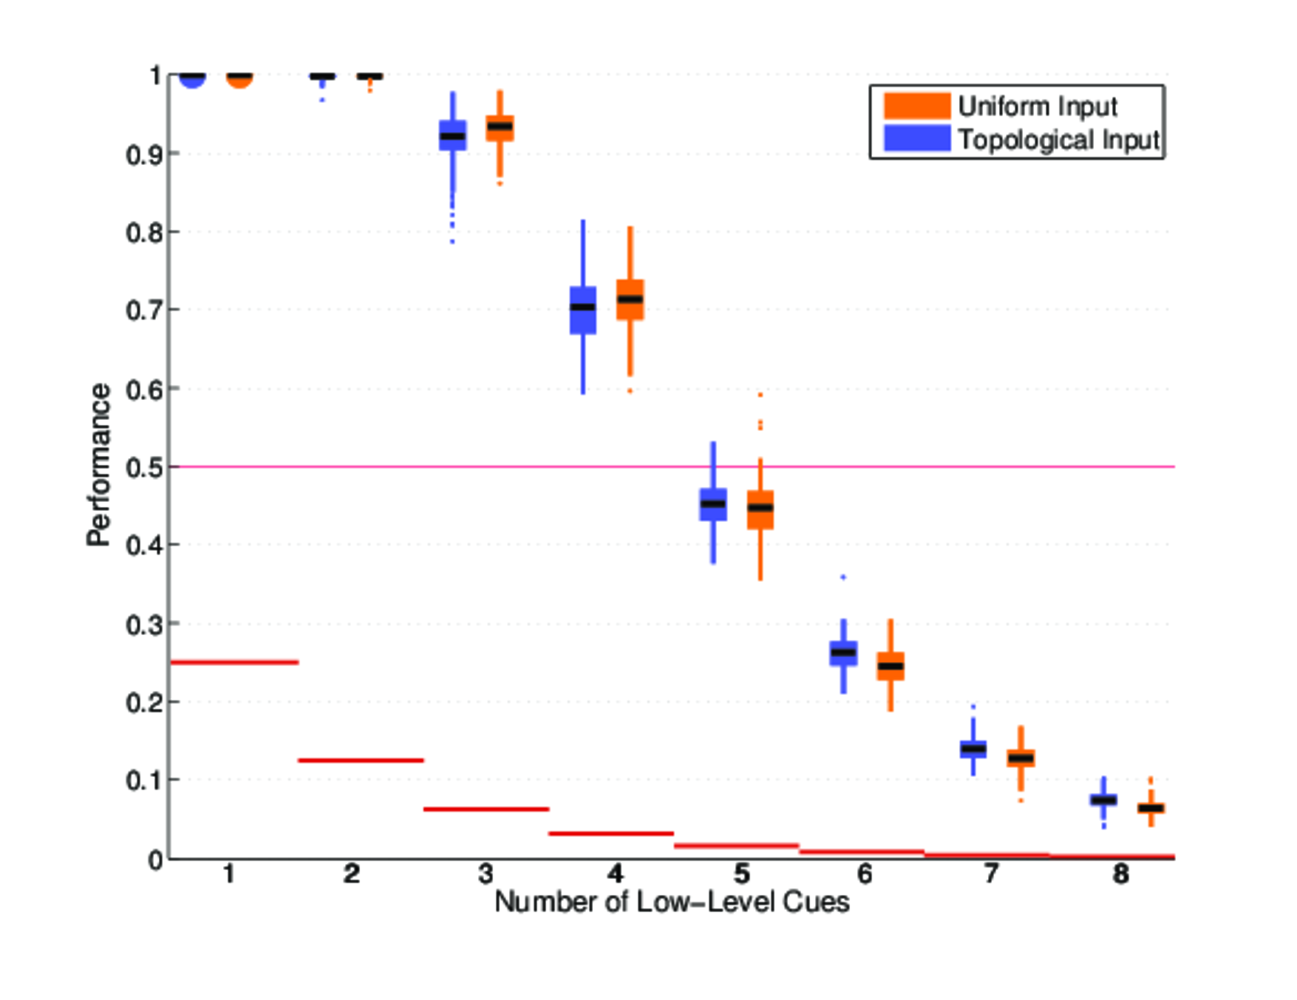
\includegraphics[width=\textwidth]{figures/polboxchance.png}
\caption{In this figure, each column represents the distribution of the performance of 200 random ESNs, with the box covering the lower quartile to the upper quartile and the whiskers covering 1.5 times the interquartile range. The blue bars represent ESNs with topological processing, the orange bars ESNs with uniform processing. At the left, the number of low-level cues that had to be integrated was just one, at the right it was eight. Obviously, the performance decreases from perfect in the easiest condition to rather low in the hardest condition. However, we also found a difference between the uniform processing ESNs and the topological processing ESNs, which is highlighted in the next figure. The red lines are at chance level for each of the conditions, while the pink line is at the performance level that can be reached by integrating all low-level cues but ignoring the high-level cue.}
\label{policyabstraction}
\end{figure}


\begin{figure}[bthp]
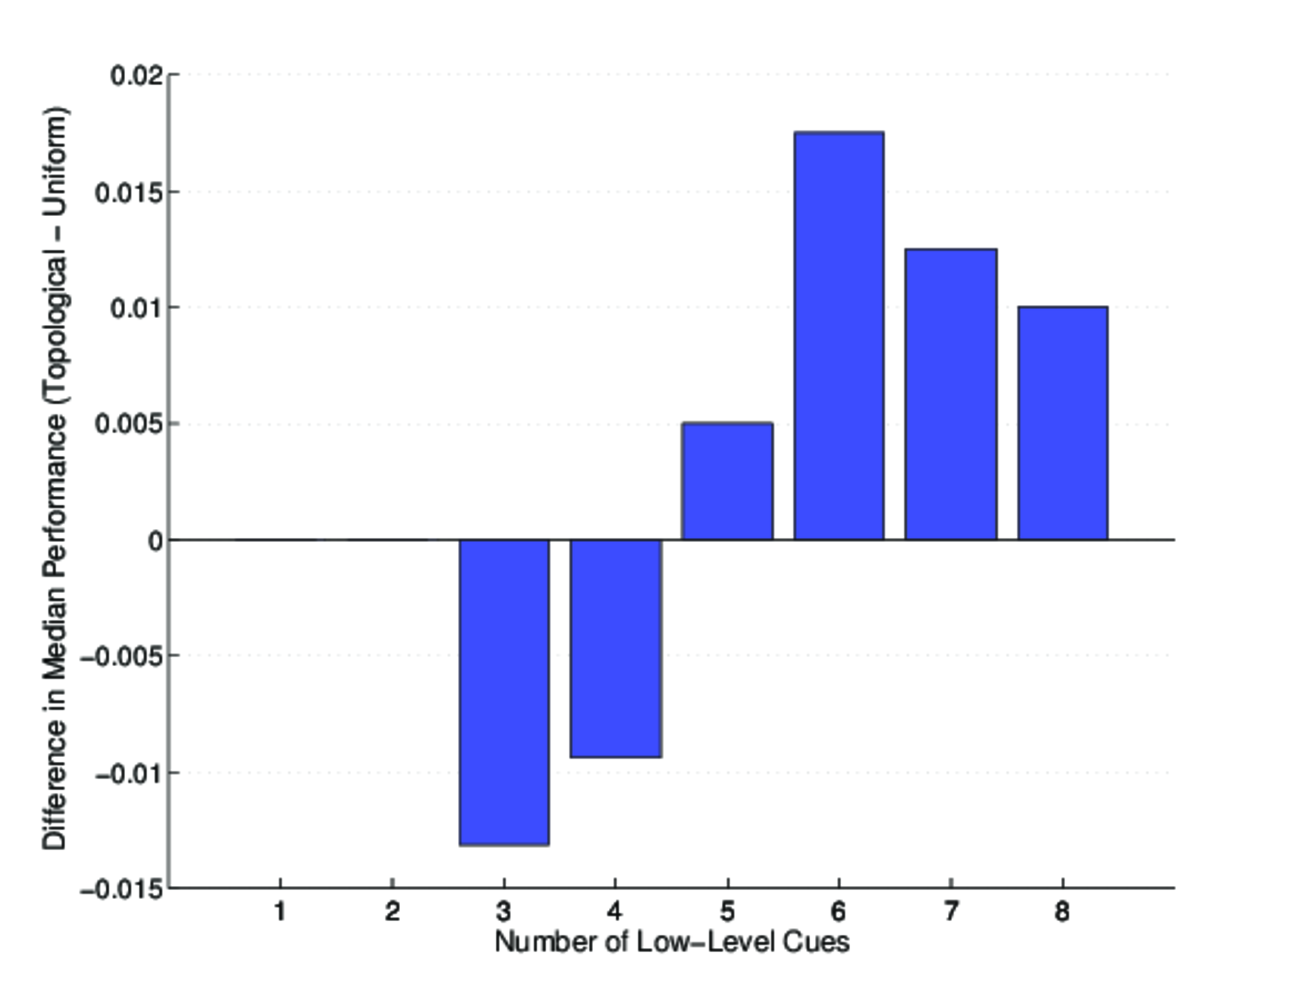
\includegraphics[width=\textwidth]{figures/polbar.png}
\caption{The difference in median performances between topological processing ESNs and uniform processing ESNs (a positive number means that the topological processing ESN performs better). From left to right the number of low level cues in the policy abstraction task is increased from one to eight. In the easiest condition, we see no difference between the network because both perform perfect. Likewise, in the hardest condition we see only a small difference because both network perform rather bad. However, in between those two extremes we see that for a smaller number of low-level cues a uniform processing network performs better, while for a larger number of low-level cues the topological processing ESN performs better.}
\label{policyabstractionbar}
\end{figure}

In figure \ref{policyabstraction} we can find the performances of the networks on the policy abstraction task. We can see that in case of a small number of low-level cues the performance of both networks is near perfect. This means that our performance measure is not suitable to find a difference in performance between the two networks in this condition. When the number of low-level cues is increased, the task apparently gets harder to solve, as the performance decreases. When eight or more low-level cues had to be integrated, the performance was very low, again limiting our ability to measure the difference between the two networks.

In figure \ref{policyabstractionbar} we can see the differences between the median performances of the networks with topological input and the networks with uniform input. As we just established, we cannot find large differences in the easiest and in the hardest condition. Over the conditions in which our performance measure gives a useful result, we see that the number of low-level cues in the WCS task is critical for the performance difference between uniform and topological networks. When a small number of features has to be integrated, the uniform network has an advantage over the topological network. However, when a large number of features has to be integrated, the performance is better when using a topological network.


\begin{figure}[bthp]
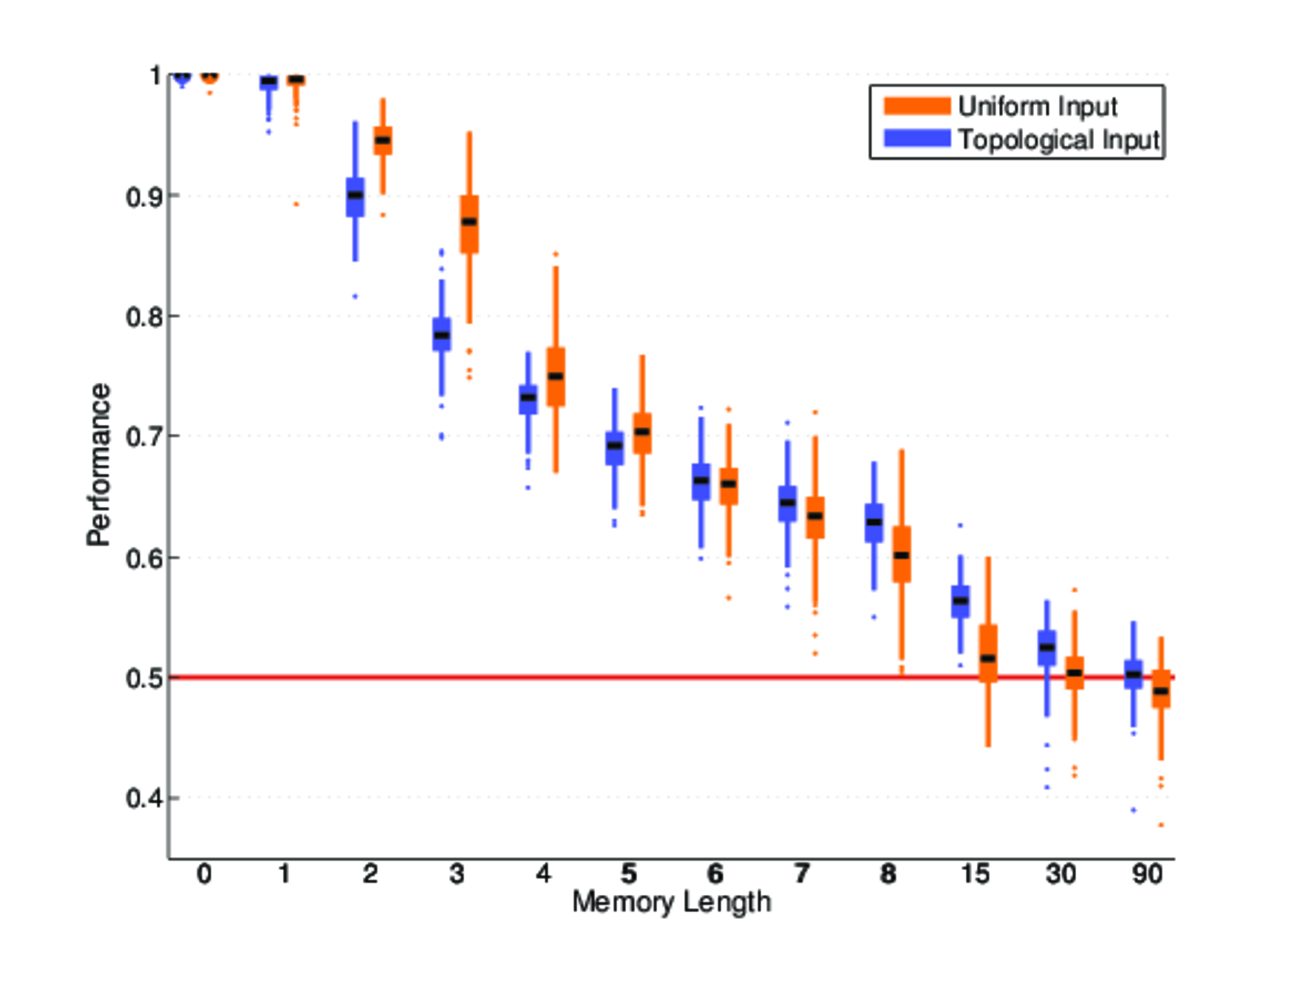
\includegraphics[width=\textwidth]{figures/memboxchance.png}
\caption{Again, each column represents the distribution of the performance of 200 random ESNs, with the box covering the lower quartile to the upper quartile and the whiskers covering 1.5 times the interquartile range. The memory length in the n-back test was increased from 0 (at the left) to 90 (at the right); note that the at the right side of the graph the steps in memory length are much larger than at the left side of the graph. Again, we can clearly see the performance decrease when the task gets harder, effectively going down to the chance level of 0.5 (the red line) in the hardest condition. The difference between the uniform input ESN and the topological input ESN is shown in the next figure. }
\label{temporalabstraction}
\end{figure}


\begin{figure}[bthp]
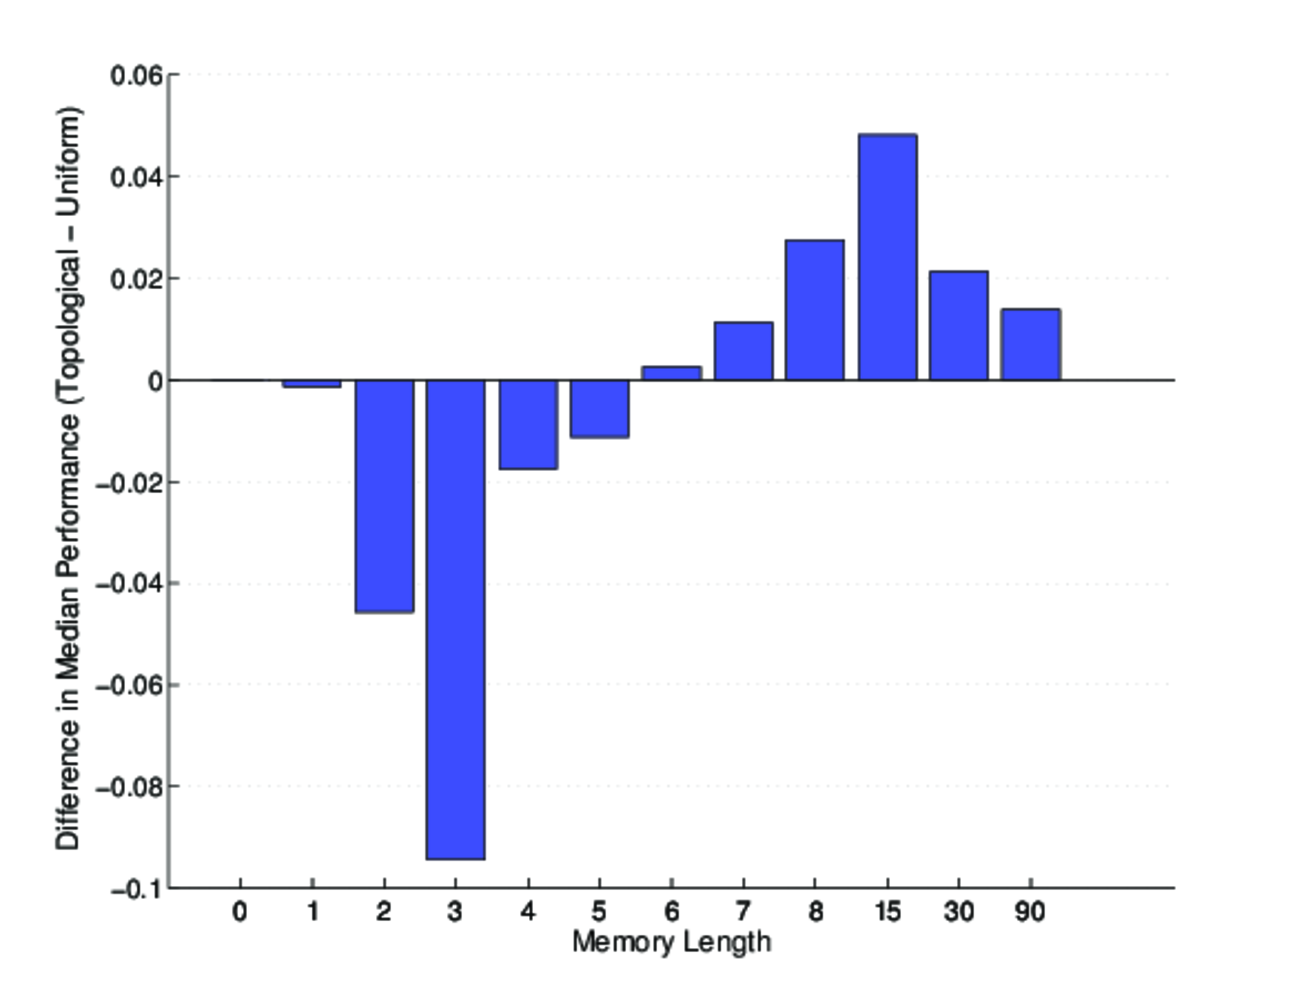
\includegraphics[width=\textwidth]{figures/membar.png}
\caption{ The difference in median performance between a uniform processing ESN and a topological processing ESN as a function of the memory length in a n-back test. At the left, the memory length is zero (which is a task without abstraction) and both performances are near perfect, making the difference between the performances small. At memory length three however, we can see that the ESN with uniform input clearly outperforms the ESN with topological input. When memory length increases further, this relation is reversed. At the longer memory lengths the difference diminishes again, because both performances drop to chance level (albeit that the topological processing ESN drops slower). Again, mind the larger steps in memory length at the right side of the graph. }
\label{temporalabstractionbar}
\end{figure}

With respect to the temporal abstraction, we can find a similar relation. In figures \ref{temporalabstraction} and \ref{temporalabstractionbar} we can see that for short memory length, uniform processing gives an advantage, while for a long memory length topological processing gives an advantage. Again we can also see that for the easiest and hardest conditions the performance measure fails to show a difference because the performance is near perfect and near chance level, respectively. Note that the measured effect in the case of temporal abstraction is much larger than in the case of policy abstraction. Also note that the easiest condition, with memory length 0, is a task without abstraction: it is purely the lookup of the current input pattern.

Significance of the results was tested with a Mann Whitney U test (also known as the Wilcoxon rank-sum test) in the conditions that showed the largest difference between the uniform and topological ESN (thus, in the conditions with 3 and 6 low level cues and in the conditions with a memory length of 3 and 15). In all these conditions, the differences between the uniform and topological ESN were highly significant, with p $<$ 0.001. Note that while it is possible to argue that the Mann Whitney U test is in fact only measuring the significance of the difference in medians under the condition that the two distribution are merely shifted, this should not affect our results because visual inspection of figure \ref{temporalabstraction} and \ref{policyabstraction} shows that the distributions are reasonably close to normal.

\section{Interpreting the Results for the PFC and the Human Brain}

The results are exactly in line with what we would expect from the hypothesis that functional localization in neural networks helps to preserve important information, but is disadvantageous for information integration: with a large number of low-level cues that have to be integrated, preserving the high-level cue to influence the low-level cues enough is more important than with a small number of low-level cues. Thus, in this situation the ESN with topological input performs better. With a small number of low-level cues on the other hand, the performance is mostly influenced by how easily the high- and low-level cues are integrated, and we see that the uniform ESN performs better. A similar explanation can be given for the n-back results: when the performance is mainly dependent on the ability to retain information (a long memory length), it is best to process information in separate locations. On the other hand, in a task with a short memory length the performance is mainly dependent on the ability to integrate information and it is best to process information uniformly. The performance of the network is therefore a trade-off between information integration and information preservation. 

The results for the mapping of temporal abstraction levels are in general agreement with other research that we discussed earlier: it has already been shown that a topological map of temporal abstraction can be the result of the backpropagation through time learning algorithm in a hierarchical network with an abstract task \citep{Botvinick2007}. Also, such a structure has been shown to partly self-organize using an evolutionary algorithm \citep{Paine2005}. The results for the mapping of policy abstraction are for example in line with the study by \citet{Yamashita2008}, which found motor primitives that could be used again in a different context. However, we go one step further than observing the topological organizations: we try to give an explanation.

We argued that we can make the step from our artificial networks to biological neural networks, because the wiring economy principle ensures that information integration is handled within areas while information that has to be preserved is processed in a separate area \citep{Sporns2010}. Indeed, we can find examples of brain structures that are in agreement with our results. The obvious example for temporal abstraction is the classical psychological distinction between short-term and long-term memory. While the debate is still out on the exact neural substrates of these memory systems, it is well-established that they are implemented using different mechanisms \citep{Eichenbaum2000}. Another example is the distinction between information that is directly used for motor actions in sensory-motor loops and information that is stored in working or short-term memory \citep{Fuster2001}. Functional specialization at different policy abstraction levels can also be found. The DLPFC exerts control over brain areas that function at lower abstraction levels, for example the premotor cortex \citep{Koechlin2003}. Indeed, those lower abstraction levels most likely have to deal with a large amount of information, e.g. sensorimotor loops or different sensor modalities, so that this mapping is beneficial according to our results (note, however, that there may be other explanations for these structures as well; also see the pitfalls section).

It is important to note that our results apply to reasonably large-scale neural networks. While a great deal is known about single neurons and small-scale neural networks, it is problematic to interpret fMRI results in those terms \citep{Nir2007, Sirotin2009}, or even to explain neural population dynamics with it \citep{Tiesinga2008, Wang2010, Belitski2008}. Therefore, studying the properties of large-scale neural networks directly can be of use. In our case, we can compare our results with the imaging studies of PFC that we discussed earlier. While our results do not cover all aspects of the PFC, we still would like to propose that the topological mapping of temporal and policy abstraction levels over the PFC is explained by the information preservation versus integration trade-off. If this is true, we expect to see similar fMRI results for tasks involving multiple levels of policy abstraction as for tasks involving multiple levels of temporal abstraction.

As we discussed in the literature review, most neuroimaging results suggest both temporal abstraction mapping and policy abstraction mapping \citep{Badre2009}. The work by \citet{Koechlin2003} is in agreement with our results, because his experiments included a large difference in timescales: the context had to be remembered for mere seconds, while the episodic control signal had to be remembered for a much longer time, in the order of minutes. This seems reasonable for tasks in daily life as well. The work by \citet{Badre2007} is slightly more difficult to explain: contrary to our findings, they find a mapping of abstraction while the number of low-level cues is small. However, this may be caused by the difference between natural tasks, that influence the structure of the brain through evolution and development, and artificial tasks used in experiments. We will discuss opportunities in this direction in the further research section. Also see the pitfalls section for alternative explanations. 

Another issue is the inconsistency between the various imaging experiments: while we predict that temporal and policy abstraction levels should lead to similar subsequent activation patterns in fMRI, the experiments have so far always involved mixtures of different abstractions. The exception is the study by \citet{Christoff2009}, but unfortunately it is in the language domain instead of the action domain. We can use it as an example for future fMRI studies though: one study assessing the different abstractions, neatly separated, could greatly benefit our understanding of the neural substrates that process abstractions. 

The most recent addition to the debate was made by \citet{Reynolds2012}. The authors argue that they did not find any evidence for topological mapping of abstraction, but propose the ``adaptive context maintenance'' hypothesis. However, they do mention that their hypothesis does not in principle exclude the cascade model proposed by \citet{Koechlin2003}. Even though our ideas are quite similar to the ideas in \citet{Reynolds2012}, our results do not agree with their conclusions. While they suggest an absence of topological mapping of abstractions, we show that we have theoretical reasons to expect it. This is regardless of how the information in the PFC is exactly maintained. As the analysis of their results is performed differently from the other studies, we suggest that the data set should be examined closer and the experiments reproduced. Also, the tasks and the strategy that people use to solve the tasks should be considered, as detailed in the literature review section.

All in all, we found one mechanism that may have driven the development of functional specialization of brain areas at different levels of policy and temporal abstraction, both in the PFC as in other brain areas. If this mechanism is indeed important for PFC development, we can explain the mapping of abstractions as proposed by \citet{Koechlin2003} and \citet{Badre2007}. Also, we predict that the tasks involving temporal and policy abstraction activate a similar sequence of PFC areas. Furthermore, we cast doubt on the proposal to do away with topological mappings of abstractions by \citet{Reynolds2012}. Of course, a model cannot change imaging results. Therefore, we proposed further investigations of the PFC; especially because the studies and evidence so far are not consistent. We will discuss promising directions for such investigations in the further research section.

\section{Pitfalls in the Interpretation}

%scale and scope
%perhaps reorganize

The first question one always has to ask in a modelling study is whether the generalization from the model to reality can be made. In our case, the first step in the generalization is the step from the ESNs we investigated to ESNs and artificial neural networks in general. Of course, we investigated a range of parameters, but due to the nature of the network and the task, the effect could not be confirmed under all parameter settings. For example, the performance could be perfect or at chance level for both networks, or one of the networks could be better regardless of the memory length or number of low level cues. In this last situation, we could not simply take the difference between the medians of the performances, because this measure could be distorted by the way we measure the performance. This gives us two possible ways in which the interpretation of our results may not be valid for neural networks in general and the brain in particular.

The first and foremost problem is that the found relation may be dependent on the parameters that we used. It is easy to assume that all relations are additive and independent of the parameters, but the fact that we are dealing with a highly non-linear system already suggests that this does not have to be true. In fact, it might be possible that under other circumstances the findings would be opposite. More simulation work could make this problem smaller, but not solve it without an exhaustive search. The second, related problem is that we only investigated a very small subset of the potential ways in which a task and the input and processing topology can interact. This means that even if the effect that we found is the same under all parameter settings, other effects may be much bigger. So, under other parameter settings or task conditions, the measured relation may only give an insignificant contribution to the total difference in performance. An example of this effect is that we had to carefully tune one parameter, namely the connection strength between the two layers of the network, to be able to find the presented results. These two problems can be mitigated by using artificial evolution, as will be described in the further research section.

The next step is to generalize our results to biological neural networks. As with many other neural networks models of the brain, an important problem is that biological neural networks are much richer than most artificial neural networks. Different neuron types, many more connections, plasticity and even signals that are propagated outside neurons, even the simple fact that real neurons have a location, all make that an artificial neural network may be insufficient to model the mechanisms of biological neural networks \citep{Anderson1995}. Moreover, we choose the task for the neural network based on current neuroscience theories, but that does not mean that the biological neural networks solve only this task: they may have other tasks as well and perhaps not do the task we used for the model at all. Obviously, the only way to solve these problem is to validate the results in biological neural networks, which will shortly be discussed in the further research section.

When applying our results to the biological neural networks in the DLPFC we encounter the specific instantiations of the general problems mentioned above. The first thing to be discussed are the parameter settings: the parameters we choose were not based on physiological results. As described above, this might make our result irrelevant for the situation in the DLPFC. In particular, we have to mention the connection strength between the top and bottom layer in our model, as this parameter turned out to be very important: changing this parameter from small to big could change an overall performance advantage for uniform networks to an overall performance advantage for topological network. While we may argue that the parameter setting we used is probably realistic, it is likely that the parameter is in fact tuned to benefit either topological or uniform processing. Physiological studies would be required to find a realistic value for the top-down connectivity. Of course, there may be other important factors in the model, that we did not investigate, as well.

%maybe at a graph describing the effect of this parameter?
%a weak top down connection benefits result in large number of low level cues conditions?

The second and arguably most important problem with applying our results to the DLPFC is that apart from exerting cognitive control, it probably also has the function of learning task sets \citep{Sakai2008}. This is a difficult thing to achieve and may therefore also have a big influence on the structure of the PFC. In fact, some researchers have already started exploring this direction. The first results indicate that a hierarchical PFC makes learning easier. In particular, it might support generalization of knowledge or task sets to new domains \citep{Reynolds2009}. This direction of research seems very promising and deserves more thorough investigations. Unfortunately, learning is out of the scope of our study as an ESN is arguably not suitable for modelling learning in the PFC.

A third interesting point is that biological neural networks may be decoupled, even when they share the same location and space. This can for example be achieved by axons preferentially attaching to a specific type of neurons. Thus, it would even be possible to construct a hierarchy in a single place, making it undetectable for fMRI. However, space is of course not unlimited in the human brain, making such a construct unlikely when larger numbers of neurons are involved: it would require longer axons than segregating the two networks. Nevertheless, small-scale hierarchies may be more common than expected and our findings are not exclusively tied to networks that are spatially segregated.

Finally, we have to ask the question whether our task matches the task that the PFC has to perform for cognitive control. An important factor is the representation of abstract information in the PFC. We used one symbolic node for each input cue in the model, with each node loosely representing a population of neurons. However, it might be the case that in the prefrontal cortex the same population of neurons is used to represent different types of information, or the opposite that multiple populations code for one particular input. This may be of influence on the results, especially because the number of relevant input nodes is one of the identified critical factors. The neural representation is an active area of research, but unfortunately not much is known yet \citep{Jin2009,Tiesinga2008}. Additionally, we only took into account temporal and policy abstraction. Badre identified two additional abstraction types: domain generality and relation integration \citep{Badre2009}. It remains to be seen whether these abstractions rely on the same general principles as we have identified here or introduce new complications that negate the current findings. Also, the full scope of the tasks of the PFC may only be investigated with embedded, embodied research; see the further research section. 

Keeping all these pitfalls in mind, we have to take great care when applying our results to biological neural networks. We have shown that functional specialization on different abstraction levels can help cognitive control, but this does not mean that this is or was in fact the case in the PFC. As we have discussed in this section, there is a handful of good reasons not to think so. However, it might be possible to show that general, structural rules of thumb can explain brain structures by doing more research.

\section{Future Research}

We will start with the most obvious idea for further research: the tasks that have been used in the past by Badre, Reynolds and Koechlin should be improved. Already, different researchers come to different results and note that this might have to do with small differences in the tasks. For example, Reynolds presented the cues for his policy abstraction tasks sequentially \citep{Reynolds2012}, while Badre presented them simultaneously \citep{Badre2007}. This means that the brain might use different ways to solve these problems possibly leading to different imaging results. When doing imaging research, we should also take the strategy that people are using into account when interpreting the results. For example, Reynolds policy abstraction task can be solved without using any abstraction, just by counting particular cues (because all cues are equally important) and then deciding whether the number is odd or even. If people indeed used such an alternative strategy, Reynolds measured something different than he thought. Thus, before testing the tasks should be carefully evaluated and in the best case be matched with earlier research. Without such an effort it will remain unclear which results are replicable and which are not.

Modelling work as has been done by \citet{Botvinick2007}, \citet{O'Reilly2006} and us, gives a different, unique possibility to improve on the tasks used so far: the models can be implemented for a robot to investigate tasks that humans and other animals have to solve in daily life. Our model has been specifically designed with this possibility in mind and it should therefore be possible to do this without much effort. This addresses the problem that the imaging results so far may be just an epiphenomenon of a different, more important structure. It has for example already been mentioned that different types of abstraction may co-occur in nature \citep{Botvinick2007}. So, an embodied platform can help to better understand the reasons why the PFC shows a certain organization, by clarifying which task the PFC actually has to solve.

Another approach to further research is to integrate information from different research areas more thoroughly. Physiological data of the brain areas under investigation is sparse, while it will be of vital importance for more detailed modelling attempts. One of the recent developments that may turn out to be important is the interest in connectomes: maps of the connections in the brain \citep{Sporns2011}. Another field that may contribute is developmental neuroscience, see for example \citet{Supekar2009} and \citet{Diamond2002} for publications in this field. Of course, evolutionary biology may contribute important insights as well: we share the general structure of our brain with all vertebrates and it is critical for our survival, suggesting slow and incremental evolution. See for example \citet{Jarvis2005} and \citet{Dunbar2007}. Physiological studies are also important: in our model, they could for example give a realistic parameter setting for top-down connectivity. Finally, we have to mention \citet{Tononi2003}: a more mathematical approach can help to quantify findings, at least in models. Whether this can be feasible in vivo remains to be seen. Interestingly, \citet{O'Reilly2006} and \citet{Hazy2007} seem to be on the right way already: their model explicitly bridges the gap between functions and brain areas and in a way approaches the PFC as an evolutionary extension to the Basal Ganglia. 

On the side of our ESNs, an important possibility is to use evolutionary algorithms. Evolutionary algorithms can cover the whole parameter space, addressing the problem that the found relations may only be valid for a small parameter range. Thus, the performances of the respective networks in our study could then be directly compared. The most interesting approach is probably to use the evolutionary algorithm not only for the parameter settings, but also for evolution of the input weights. This way, we can directly evaluate whether the benefits of topological mapping can indeed drive evolution and self-organize the ESN into a hierarchy with specializations at different abstraction levels. This would in fact be a logical extension of the work of \citet{Paine2005}: they showed that a network adapts its time constants when input is giving at different locations, but not the reverse. It would be similar with the research of \citet{Botvinick2007}, but with an unsupervised learning method instead of a lengthy supervised learning method. Also see \citet{Bullinaria2009} for additional thoughts on computational modelling of brain structures.

One could also attempt to explicitly model the PFC with an ESN. Earlier, we noted that this was not the ideal interpretation of our research, but it is not impossible. It will require some creative work though, as it is not directly obvious how to relate the performance of the ESN to behavioural measures. Also, before trying to do this one has to take into account that there are already many other models that were made to match behaviour on a large range of psychological tests, for example the cognitive architectures \citep{Anderson1997}. To take an extra step in this direction it is probably a better idea to use or improve one of the existing other models. On the other hand, an explicit match of our results with behavioural results would make the claim that the PFC shows functional specialization on different abstraction levels, because it improves cognitive control, much more plausible.

Also, such a model would be unique in its capability to directly investigate structure and hierarchy. This can be useful to model recent findings of changed connectivity patterns: healthy people showed a hierarchical organization of the multimodal network (as we described earlier), while this hierarchy was reduced in people with schizophrenia \citep{Bassett2008}. Interestingly, schizophrenia also compromises the performance on certain cognitive control tasks. Particularly, the masking paradigm (in which a very short stimulus is preceded or succeeded by a mask) shows that patients have a deficit in top-down control of visual information processing \citep{Gilbert2007}. Thus, it may be possible to link the control deficits with the change in PFC organization by using an ESN-based model. Other diseases, like Alzheimer's disease, may be investigated in a similar way \citep{Sporns2011a}.

Finally, we would like to include some notes on further research that would be necessary to use our model successfully as a robot controller. Arguably the best way to do this, is to embed the ESN in a behaviour that is part of a larger behavioural system. The input to this behaviour can be an arbitrary set of sensor signals, while the output of the ESN can be used to influence the other behaviours (e.g. just by increasing or decreasing its importance during action selection). The ESN can then be compared with a classifier of contexts in which particular behaviours are relevant, or with an affordance calculator \citep{Scheutz2004}. The benefit compared to existing solutions would be that we can use a recurrent neural network to do this classification automatically (with supervised training). The foremost problem that should be solved for this application is that we want to use analog and continuous input signals while our research only employed binary input signals at fixed time intervals. While ESNs generally work with analog inputs, adapting it for continuous input might prove challenging. A different opportunity would be to investigate how performance can be increased by the choice of the reservoir and by reservoir adaptation. In our results we can already see a large spread in performance and some articles describe how to choose and adapt reservoirs \citep{Jarvis2010, Sussillo2009, Dutoit2009}.
 
Obviously, a great opportunity would be to combine evolutionary algorithms and robots for on-line evolution. It has already been shown that an evolutionary algorithm can be used to replace the regression procedure for training an ESN \cite{Hartland2009}, allowing for unsupervised learning of the whole ESN and therefore unsupervised context learning. The parameters of the network and the input weights would have to evolve at a slower time scale than the output weights to make sure that a specific output weight setting does not hamper evolution. Different outputs biasing specific behaviours would show co-evolution, as the outputs of the ESN are not directly related to one another, but only through the environment \citep{Nolfi1998}. This also means that new behaviours can be added later without too much effort, possibly addressing a major problem in behavioural robotics \citep{Arkin1998}.

\chapter{Conclusion}

All in all, we conclude that research bridging robotics, artificial intelligence and cognitive neuroscience can lead to important results. We confirmed our hypothesis that cognitive control tasks with temporal and policy abstraction share the same requirements regarding information separation and preservation: within each abstraction level information integration is most important, while between abstraction levels information preservation is most important. This finding can explain the observed topological mapping of abstraction levels in the PFC, because the wiring economy principle leads to information being integrated best in a single area and preserved best by being spatially segregated. Despite a number of limitations, especially not taking into account learning, we can still use these results to give a theoretical background for the interpretation of imaging results. Specifically, we show that the mapping of temporal and policy abstractions in the PFC may be explained by the same principles and that we have a good reason to expect a hierarchy of abstraction levels to be present, contrary to a recent proposal. 

Besides the results from the simulation, we also proposed a number of improvements on the tasks used so far. Firstly, using the traditional abstract tasks more consistently can help to clarify the discrepancies in the imaging results so far. Secondly, we constructed our model in such a way that it can be used as a robot controller for embodied and embedded research. This would allow to investigate tasks that are encountered in daily life and have structured our brain during evolution. A robot implementation of our model can also bring significant results for robotics research: it gives a way to adapt a behavioural system to the current context and information that has been integrated over time. This can make the tedious process of building a behavioural robot controller easier, as not all the different situations and interactions have to be encoded in the hand-wired connections between behaviours. Instead, the learning procedure for the Echo State Network can take this burden.

%\clearpage
%\addcontentsline{toc}{chapter}{Bibliography}
\bibliography{regulativeControl}

\appendix
\chapter{Further Technical Thoughts}

In this appendix we will give some further thoughts about the technical features of Continuous Time Echo State Networks (CTESN) and application in robots. First of all, we would like to show that the CTESN approach can indeed handle multiple timescales and has a memory length that can practically exceed the reservoir size. For this, we constructed a new task with 3 levels of abstraction. At the top level, we find one input node that gives a high value once every 600 trials. This high value (that lasts for one trial only) indicates the start of a 400-trial episode in which one of the two input nodes at the middle level is relevant. After this episode, the other input node at the middle level is relevant again. The same is true for each of the input nodes at the middle level: each of them signals the start of an episode in which one out of two input nodes at the bottom level is relevant (thus, this makes a total of four input nodes at the bottom level). These cues are given once every 30 trials and the episode lasts 20 trials. The bottom input nodes are only relevant for the current trial and the relevant node signals which output node should be chosen, giving us a total of eight output nodes. 

Note that the average value of all the input nodes is set to zero, to prevent the top and middle parts of the ESNs being driven to extreme activation values by the `standard' input value. For a robot, this might mean that the input to the higher areas of the network (with slow time constants) should be high-pass filtered, for example by calculating a running average for a sensor value and only give the difference of the current sensor value with the running average as an input to the network. This keeps successive sensor readings from driving the network to extreme activation values. Instead, input is only given when the current situation changes.

The task can be performed relatively well, even by small CTESNs. In figure \ref{3levels} the performance distributions are shown for different reservoir sizes. Note that the performance of a method without any memory would be 0.25 and the performance of a system that only handles the bottom and middle level would be 0.5 . Most of the CTESNs give a performance much better than that, even if the reservoir consists of just 60 nodes. Note that each condition contains only 20 reservoirs; the figure is only meant to illustrate the general trend. Also note that while some time was spent to tune the time constants, this performance level was reached within a couple of hours and can probably still be significantly improved. The matlab code for the tasks and the CTESN with three levels can be found at \url{https://github.com/RemcoTukker/PFC-ESN}.

\begin{figure}[bthp]
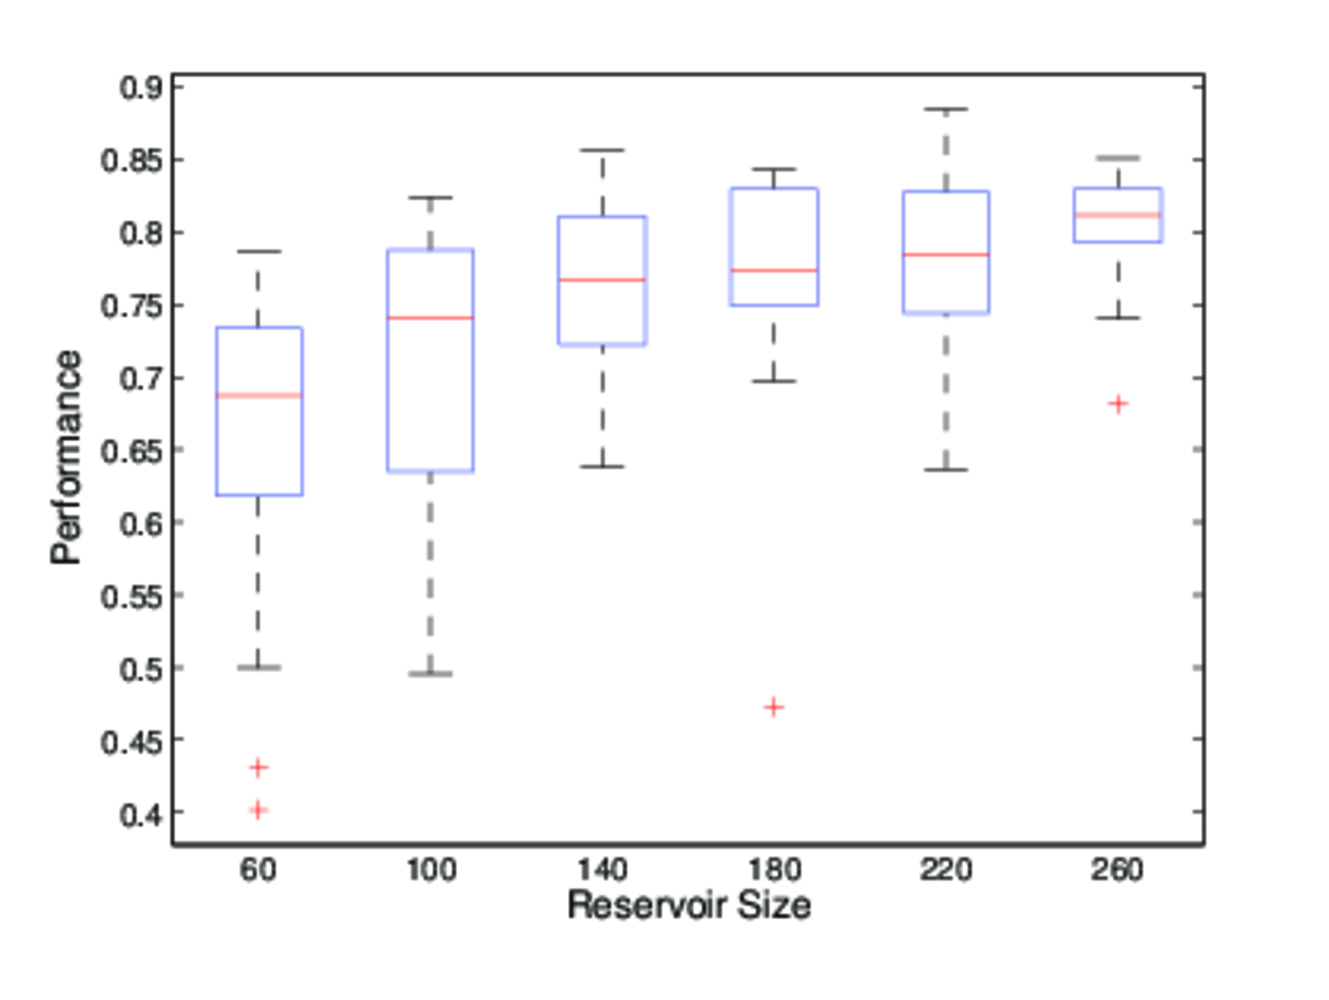
\includegraphics[width=\textwidth]{figures/3levels.png}
\caption{Each column represents the distribution of the performance of 20 random ESNs, with the box covering the lower quartile to the upper quartile and the whiskers covering 1.5 times the interquartile range.}
\label{3levels}
\end{figure}

However, we can also note that increasing the size of the reservoir gives only small improvements in performance. The cause is that most nodes that are added do in fact not contribute to the richness in the reservoir, but are instead completely redundant. One method that might solve this issue is backpropagation-decorrelation \citep{Steil2004, Steil2007}, but we lacked the time to investigate this approach.

Another opportunity is to investigate how well a support vector machine (SVM) would perform on the policy abstraction task described in this thesis. While it cannot intrinsically integrate information over time, it may well be that it outperforms the ESN on tasks that do not contain temporal abstraction. In such tasks, an SVM may be useful for classifying context in behavioural robot controllers. 

\end{document}